\documentclass[11pt,]{article}
\usepackage{lmodern}
\usepackage{amssymb,amsmath}
\usepackage{ifxetex,ifluatex}
\usepackage{fixltx2e} % provides \textsubscript
\ifnum 0\ifxetex 1\fi\ifluatex 1\fi=0 % if pdftex
  \usepackage[T1]{fontenc}
  \usepackage[utf8]{inputenc}
\else % if luatex or xelatex
  \ifxetex
    \usepackage{mathspec}
  \else
    \usepackage{fontspec}
  \fi
  \defaultfontfeatures{Ligatures=TeX,Scale=MatchLowercase}
\fi
% use upquote if available, for straight quotes in verbatim environments
\IfFileExists{upquote.sty}{\usepackage{upquote}}{}
% use microtype if available
\IfFileExists{microtype.sty}{%
\usepackage{microtype}
\UseMicrotypeSet[protrusion]{basicmath} % disable protrusion for tt fonts
}{}
\usepackage[margin=1in]{geometry}
\usepackage{hyperref}
\hypersetup{unicode=true,
            pdftitle={Effective application of machine learning to microbiome based classification problems},
            pdfborder={0 0 0},
            breaklinks=true}
\urlstyle{same}  % don't use monospace font for urls
\usepackage{graphicx,grffile}
\makeatletter
\def\maxwidth{\ifdim\Gin@nat@width>\linewidth\linewidth\else\Gin@nat@width\fi}
\def\maxheight{\ifdim\Gin@nat@height>\textheight\textheight\else\Gin@nat@height\fi}
\makeatother
% Scale images if necessary, so that they will not overflow the page
% margins by default, and it is still possible to overwrite the defaults
% using explicit options in \includegraphics[width, height, ...]{}
\setkeys{Gin}{width=\maxwidth,height=\maxheight,keepaspectratio}
\IfFileExists{parskip.sty}{%
\usepackage{parskip}
}{% else
\setlength{\parindent}{0pt}
\setlength{\parskip}{6pt plus 2pt minus 1pt}
}
\setlength{\emergencystretch}{3em}  % prevent overfull lines
\providecommand{\tightlist}{%
  \setlength{\itemsep}{0pt}\setlength{\parskip}{0pt}}
\setcounter{secnumdepth}{0}
% Redefines (sub)paragraphs to behave more like sections
\ifx\paragraph\undefined\else
\let\oldparagraph\paragraph
\renewcommand{\paragraph}[1]{\oldparagraph{#1}\mbox{}}
\fi
\ifx\subparagraph\undefined\else
\let\oldsubparagraph\subparagraph
\renewcommand{\subparagraph}[1]{\oldsubparagraph{#1}\mbox{}}
\fi

%%% Use protect on footnotes to avoid problems with footnotes in titles
\let\rmarkdownfootnote\footnote%
\def\footnote{\protect\rmarkdownfootnote}

%%% Change title format to be more compact
\usepackage{titling}

% Create subtitle command for use in maketitle
\newcommand{\subtitle}[1]{
  \posttitle{
    \begin{center}\large#1\end{center}
    }
}

\setlength{\droptitle}{-2em}

  \title{\textbf{Effective application of machine learning to microbiome based
classification problems}}
    \pretitle{\vspace{\droptitle}\centering\huge}
  \posttitle{\par}
    \author{}
    \preauthor{}\postauthor{}
    \date{}
    \predate{}\postdate{}
  
\usepackage{booktabs}
\usepackage{longtable}
\usepackage{array}
\usepackage{multirow}
\usepackage[table]{xcolor}
\usepackage{wrapfig}
\usepackage{float}
\usepackage{colortbl}
\usepackage{pdflscape}
\usepackage{tabu}
\usepackage{threeparttable}
\usepackage{threeparttablex}
\usepackage[normalem]{ulem}
\usepackage{makecell}
\usepackage{caption}
\usepackage{hyperref}
\usepackage{helvet} % Helvetica font
\renewcommand*\familydefault{\sfdefault} % Use the sans serif version of the font
\usepackage[T1]{fontenc}
\usepackage[labelfont=bf]{caption}

\usepackage[none]{hyphenat}

\usepackage{setspace}
\doublespacing
\setlength{\parskip}{1em}

\usepackage{lineno}

\usepackage{pdfpages}
\floatplacement{figure}{H} % Keep the figure up top of the page

\begin{document}
\maketitle

\vspace{35mm}

Running title: Machine learning methods applied to microbiome studies

\vspace{35mm}

Begüm D. Topçuoğlu\({^1}\), Nicholas A. Lesniak\({^1}\), Mack
Ruffin\({^3}\), Jenna Wiens\({^2}\), Patrick D.
Schloss\textsuperscript{1\(\dagger\)}

\vspace{38mm}

\(\dagger\) To whom correspondence should be addressed:
\href{mailto:pschloss@umich.edu}{\nolinkurl{pschloss@umich.edu}},
\href{mailto:wiensj@umich.edu}{\nolinkurl{wiensj@umich.edu}}

1. Department of Microbiology and Immunology, University of Michigan,
Ann Arbor, MI 48109

2. Department of Electrical Engineering and Computer Science, University
or Michigan, Ann Arbor, MI 48109

3. Department of Family Medicine and Community Medicine, Penn State
Hershey Medical Center, Hershey, PA

\newpage

\linenumbers

\subsection{Abstract}\label{abstract}

Machine learning (ML) modeling of the human microbiome has the potential
to identify microbial biomarkers and aid in diagnosis of many diseases
such as inflammatory bowel disease, diabetes, and colorectal cancer.
Progress has been made towards developing ML models that predict health
outcomes using bacterial abundances, but inconsistent adoption of
training and evaluation methods call the validity of these models into
question. Furthermore, there appears to be a preference by many
researchers to favor increased model complexity over interpretability.
To overcome these challenges, we trained seven models that used fecal
16S rRNA sequence data to predict the presence of colonic screen
relevant neoplasias (SRNs; n=490 patients, 261 controls and 229 cases).
We developed a reusable open-source pipeline to train, validate and
interpret the models. To show the effect of model selection, we assessed
the predictive performance, interpretability, and training time of
L2-regularized logistic regression, L1 and L2-regularized support vector
machines (SVM) with linear and radial basis function kernels, decision
trees, random forest, and gradient boosted trees (XGBoost). The random
forest model performed best at detecting SRNs with an AUROC of 0.695
{[}IQR 0.651-0.739{]} but was slow to train (83.2 h) and not immidiately
interpretable. Despite its simplicity, L2-regularized logistic
regression followed random forest in predictive performance with an
AUROC of 0.680 {[}IQR 0.625-0.735{]}, trained faster (12 min), and
yielded a model that was inherently interpretable. Our analysis
highlights the importance of choosing an ML approach based on the goal
of the study, as the choice will inform expectations of performance and
interpretability.

\newpage

\subsection{Importance}\label{importance}

Prediction of health outcomes using machine learning (ML) is rapidly
being adopted in microbiome studies. However, estimated performance
associated with these ML models is likely overoptimistic. Moreover,
there is a trend towards using black box models without a discussion of
the difficulty of interpreting such models when trying to identify
microbial biomarkers of disease. This work represents a step towards
developing more reproducble ML practices in applying ML to microbiome
research. We implement a rigorous pipeline and emphasize the importance
of selecting ML models that reflect the goal of the study. These
concepts are not particular to the study of health outcomes but can also
be applied to environmental microbiology studies.

\newpage

\subsection{Background}\label{background}

As the number of people represented in human microbiome datasets grow,
there is an increasing desire to use microbiome data to diagnose
disease. However, the structure of the human microbiome is remarkably
variable among individuals to the point where it is often difficult to
identify the bacterial populations that are associated with diseases
using traditional statistical models. This variation is likely due to
the ability of many bacterial populations to fill the same niche such
that different populations cause the same disease in different
individuals. Furthermore, a growing number of studies have shown that it
is rare for a single bacterial species to be associated with a disease.
Instead, subsets of the microbiome account for differences in health.
Traditional statistical approaches do not adequately account for the
variation in the human microbiome and typically consider the protective
or risk effects of each bacterial population seperately (1). Recently,
machine learning (ML) models have grown in popularity among microbiome
researchers as our ability to to sample large numbers of individuals has
grown; such models can effectively account for the interpersonal
microbiome variation and the ecology of disease.

ML models can be used to increase our understanding of the variation in
the structure of existing data and in making predictions about new data.
Researchers have used ML models to diagnose and understand the
ecological basis of diseases such as liver cirrhosis, colorectal cancer,
inflammatory bowel diseases, obesity, and type 2 diabetes (2--19). The
task of diagnosing an individual relies on a rigorously validated model.
However, there are common methodological and reporting problems that
arise when applying ML to such data, that need to be addressed for the
field to progress. These problems include a lack of transparency in
which methods are used and how these methods are implemented; evaluating
models without a separate held-out test data; unreported variation
between the predictive performance on different folds of
cross-validation; and unreported variation between cross-validation and
testing performances. Though, the microbiome field is making progress to
avoid some of these pitfalls including validating their models on
independent datasets (8, 19, 20) and introducing ways to better use ML
tools (21--24), more work is needed to further improve reproducibility
and minimize overestimating for model performance.

Among microbiome researchers, the lack of justification when selecting a
modeling approach has often been due to an implicit assumption that more
complex models are better. This has resulted in a trend towards using
non-linear models such as random forest and deep neural networks (3, 12,
25--27) over simpler models such as logistic regression or other linear
models (19, 23, 28). Although in some cases complex models may capture
important non-linear relationships and therefore yield better
predictions, they can also result in black boxes that lack
interpretability. Such models require post hoc explanations to quantify
the importance of each feature in making predictions. Depending on the
goal of the modeling, other approaches may be more appropriate. For
example, researchers trying to identify the microbiota associated with
disease may desire a more interpretable model, whereas clinicians may
(but not always) emphasize predictive performance. Nonetheless, it is
important to understand that the benefit of more complex, less
interpretable models may be minimal (29, 30). It is important for
researchers to justify their choice of modeling approach.

To showcase a rigorous ML pipeline and to shed light on how ML model
selection can affect modeling results, we performed an empirical
analysis comparing seven modeling approaches with the same dataset and
pipeline. We built three linear models with different forms of
regularization: L2-regularized logistic regression and L1 and
L2-regularized support vector machines (SVM) with a linear kernel. We
also trained four non-linear models: SVM with radial basis function
kernel, a decision tree, random forest and gradient boosted trees. We
compared their predictive performance, interpretability, and training
time. To demonstrate the performance of these modeling approaches and
our pipeline, we used data from a previously published study that sought
to classify individuals as having normal colons or colonic lesions based
on the 16S rRNA gene sequences collected from fecal samples (4). This
dataset was selected because it is a relatively large collection of
individuals (N=490) connected to a clinically significant disease where
there is ample evidence that the disease is driven by variation in the
microbiome (2, 4, 5, 31). With this dataset, we developed an ML pipeline
that can be used in many different scenarios for training and evaluating
models. This framework can be easily applied to other host-associated
and environmental microbiome datasets.

\subsection{Results}\label{results}

\textbf{Model selection and pipeline construction}. We established a
reusable ML pipeline for model selection and evaluation, focusing on
seven different commonly used supervised learning algorithms {[}Figure
1{]}.

First, we randomly split the data into training and test sets so that
the training set consisted of 80\% of the full dataset, while the test
set was composed of the remaining 20\% {[}Figure 1{]}. To maintain the
distribution of controls and cases found in the full dataset, we
performed stratified splits. For example, our full dataset included 490
individuals. Of these, 261 had normal colons (53\%) and 229 had a screen
relevant neoplasia (SRN; 46.7\%). A training set included 393
individuals, of which 209 had an SRN (53\%), while the test set was
composed of 97 individuals of which 52 had an SRN (54\%). The training
data were used to build and select the models and the test set was used
for evaluating the model.

We trained seven different models using the training data {[}Table 1{]}.
We focused on different classification algorithms and regularization
methods. Regularization helps to prevent overfitting by penalizing a
model that fits the training data too well (32). For regularized
logistic regression and SVM with a linear kernel, we used
L2-regularization to keep all potentially important features. For
comparison, we also trained an L1-regularized SVM with a linear kernel.
L1-regularization on microbiome data led to a sparser solution (i.e.,
forced many coefficients to zero). To explore the potential for
non-linear relationships among features to improve classification, we
trained tree-based models including a decision tree, a random forest,
and gradient boosted trees (XGBoost) and an SVM with a non-linear
kernel.

Model selection requires tuning hyperparameters. Hyperparameters are
parameters that need to be specified or tuned by the user, in order to
train a model for a specific modeling problem. For example, when using
regularization, C is a hyperparameter that indicates the penalty for
overfitting. Hyperparameters are tuned using the training data to find
the best model. We selected hyperparameters by performing repeated
five-fold cross-validation (CV) on the training set {[}Figure 1{]}. The
five-fold CV was also stratified to maintain the overall case and
control distribution. We chose the hyperparameter values that led to the
best average CV predictive performance using the area under the receiver
operating characteristic curve (AUROC) {[}Figure S1 and S2{]}. The AUROC
ranges from 0, where the model's predictions are perfectly incorrect, to
1.0, where the model perfectly distinguishes between cases and controls.
An AUROC value of 0.5 indicates that model's predictions are no
different than random. To select hyperparameters, we performed a grid
search for hyperparameter settings when training the models. Default
hyperparameter settings in previously developed ML packages available in
R, Python, and MATLAB programming languages may be inadequate for
effective application of classification algorithms and should to be
optimized for each new ML task. For example, L1-regularized SVM with
linear kernel showed large variability between different regularization
strengths (C) and benefited from tuning {[}Figure S1{]}.

Once hyperparameters were selected, we trained the model using the full
training dataset and applied the final model to the held-out data to
evaluate the testing predictive performance of each model. The
data-split, hyperparameter selection, training and testing steps were
repeated 100 times to obtain a robust interpretation of model
performance, less likely to be affected by a ``lucky'' or ``unlucky''
split {[}Figure 1{]}.

\textbf{Predictive performance and generalizability of the seven
models.} We evaluated the predictive performance of the seven models to
classify individuals as having normal colons or SRNs {[}Figure 2{]}. The
predictive performance of random forest model was higher than other ML
models with a median 0.695 {[}IQR 0.650-0.739{]}, though not
significantly (p=0.5) (Figure S3). Similarly, L2-regularized logistic
regression, XGBoost, L2-regularized SVM with linear and radial basis
function kernel AUROC values were not significantly different from one
another and had median AUROC values of 0.680 {[}IQR 0.639-0.750{]},
0.679 {[}IQR 0.643-0.746{]}, 0.678 {[}IQR 0.639-0.750{]} and 0.668
{[}IQR 0.639-0.750{]}, respectively. L1-regularized SVM with linear
kernel and decision tree had significantly lower AUROC values than the
other ML models with median AUROC of 0.650 {[}IQR 0.629-0.760{]} and
0.601 {[}IQR 0.636-0.753{]}, respectively {[}Figure 2{]}. Interestingly,
these results demonstrate that the most complex model (XGBoost) did not
have the best performance and that the most interpretable models
(L2-regularized logistic regression and L2-regularized SVM with linear
kernel) performed nearly as well non-linear models.

To evaluate the generalizability of each model, we compared the median
cross-validation AUROC to the median testing AUROC. If the difference
between the cross-validation and testing AUROCs was large, then that
could indicate that the models were overfit to the training data. The
difference in median AUROCs was 0.021 in L1-regularized SVM with linear
kernel, followed by SVM with radial basis function kernel and decision
tree with a difference of 0.007 and 0.006, respectively {[}Figure 2{]}.
These differences are relatively small and give us confidence in our
estimate of the generalization performance of the models.

To evaluate the variation in the estimated performance, we calculated
the range of AUROC values for each model using 100 data-splits. The
range among the testing AUROC values within each model varied by 0.230
on average across the seven models. If we had only done a single split,
then there is a risk that we could have gotten lucky or unlucky in
estimating model performance. For instance, the lowest AUROC value of
the random forest model was 0.593 whereas the highest was 0.810. These
results showed that depending on the data-split, the testing performance
can vary {[}Figure 2{]}. Therefore, it is important to employ multiple
data splits when estimating generalization performance.

To show the effect of sample size on model generalizability, we compared
cross-validation AUROC values of L2-regularized logistic regression and
random forest models when we subsetted our original study design with
490 subjects to 15, 30, 60, 120, and 245 subjects {[}Figure S4{]}. The
variation in cross-validation performance within both models at lower
sample sizes was larger than when the full collection of samples was
used to train and validate the models. Because of the high
dimensionality of the microbiome data (6920 OTUs), large sample sizes
can lead to better models.

\textbf{Interpretation of each ML model.} Interpretability is related to
the degree to which humans can understand the reasons behind a model
prediction (33--35). Because we often use ML models not just to predict
a health outcome, but also to identify potential biomarkers for disease,
model interpretation becomes crucial for microbiome studies. ML models
often decrease in interpretability as they increase in complexity. In
this study, we used two methods to help interpret our models.

First, we interpreted the feature importance of the linear models (L1
and L2-regularized SVM with linear kernel and L2-regularized logistic
regression) using the median rank of absolute feature weights for each
OTU {[}Figure 3{]}. We also reviewed the signs of feature weights to
determine whether an OTU was associated with classifying a subject as
being healthy or having an SRN. It was encouraging that many of the
highest ranked OTUs were shared across these three models, (e.g.~OTUs
50, 426, 609, 822, 1239). The benefit of this approach was that the
results of the analysis were based on the trained model parameters and
provided information regarding the sign and magnitude of the impact of
each OTU. However, this approach is limited to linear models or models
with prespecified interaction terms.

Second, to analyze non-linear models we interpreted the feature
importance using permutation importance (36). Whereas the absolute
feature weights were determined from the trained models, here we
measured importance using the held-out test data. Permutation importance
analysis is a post hoc explanation of the model, in which we randomly
permuted groups of perfectly correlated features together and other
features individually across the two groups in the held-out test data.
We then calculated how much the predictive performance of the model
(i.e, testing AUROC values) decreased when each OTU or group of OTUs was
randomly permuted. We ranked the OTUs based on how much the median
testing AUROC decreased when it was permuted; the OTU with the largest
decrease ranked highest {[}Figure 4{]}. Among the twenty OTUs with the
largest impact, there was only one OTU (OTU 822) that was shared among
all of the models; however, we found three OTUs (OTUs 58, 110, 367) that
were important in each of the tree-based models. Similarly, the random
forest and XGBoost models, shared four of the most important OTUs (OTUs
2, 12, 361, 477). Permutation analysis results also revealed that with
the exception of the decision tree model, removal of any individual OTU
had minimal impact on model performance. For example, if OTU 367 was
permuted across the samples in the decision tree model, the median AUROC
dropped from 0.601 to 0.525. In contrast, if the same OTU was permuted
in the random forest model, the AUROC only dropped from 0.695 to 0.680
which indicated high degree of collinearity in the dataset. Permutation
analysis allowed us to gauge the importance of each OTU in non-linear
models and partially account for collinearity by grouping correlated
OTUs to determine their impact as a group.

To further highlight the differences between the two interpretation
methods, we used permutation importance to interpret the linear models
{[}Figure S5{]}. When we analyzed the L1-regularized SVM with linear
kernel model using feature rankings based on weights {[}Figure 3{]} and
permutation importance {[}Figure S5{]}, 17 of the 20 top OTUs (e.g.~OTU
609, 822, 1239) were deemed important by both interpretation methods.
Similarly, for the L2-regularized SVM and L2-regularized logistic
regression, 9 and 12 OTUs, respectively, were shared among the two
interpretation methods. These results indicate that both methods are
consistent in selecting the most important OTUs.

\textbf{The computational efficiency of each ML model.} We compared the
training times of the seven ML models. We did not take advantage of
parallelization in training nor was the code optimized for speed. Still,
as expected, the training times increased with the complexity of the
model and the number of potential hyperparameter combinations. Also, the
linear models trained faster than non-linear models {[}Figures S1-S2;
Figure 5{]}.

\subsection{Discussion}\label{discussion}

There is a growing awareness that many human diseases and environmental
processes are not driven by a single organism but are the product of
multiple bacterial populations. Traditional statistical approaches are
useful for identifying those cases where a single organism is associated
with a process. In contrast, ML methods offer the ability to incorporate
the structure of the microbial communities as a whole and identify
associations between community structure and disease state. If it is
possible to classify communities reliably, then ML methods also offer
the ability to identify those microbial populations within the
communities that are responsible for the classification. However, the
application of ML in microbiome studies is still in its infancy and the
field needs to develop a better understanding of different ML methods,
their strengths and weaknesses, and how to implement them.

To address these needs, we developed an open-sourced framework to ML
models. Using this pipeline, we benchmarked seven ML models and showed
that the tradeoff between model complexity and performance may be less
severe than originally hypothesized. In terms of predictive performance,
the random forest model had the best AUROC compared to the other six
models. However, the second-best model was L2-regularized logistic
regression with a median AUROC difference less than 0.015 compared to
random forest. While our implementation of random forest took 83.2 hours
to train, our L2-regularized logistic regression trained in 12 minutes.
In terms of interpretability, random forest is a non-linear ML model
while L2-regularized logistic regression, a linear model, is easily
interpreted according to the feature weights. Comparing many different
models showed us that the most complex model was not necessarily the
best model for our ML task.

We established a pipeline that can be generalized to any modeling method
that predicts a binary health outcome. We performed a random data-split
to create a training set (80\% of the data) and a held-out test set
(20\% of the data), which we used to evaluate predictive performance. We
repeated this data-split 100 times to measure the possible variation in
predictive performance. During training, we tuned the model
hyperparameters with a repeated five-fold cross-validation. Despite the
high number of features microbiome datasets typically have, the models
we built with this pipeline generalized to the held-out test sets.

We highlighted the importance of model interpretation to gain greater
biological insights into microbiota-associated diseases. In this study,
we showcased two different interpretation methods: ranking each OTU by
(i) their absolute weights in the trained models and (ii) their impact
on the predictive performance based on permutation importance.
Human-associated microbial communities have complex correlation
structures which create collinearity in the datasets. This can hinder
our ability to reliably interpret models because the feature weights of
correlated OTUs are influenced by one another (37). To capture all
important features, once we identify highly ranked OTUs, we should
review their relationships with other OTUs. These relationships will
help us generate new hypotheses about the ecology of the disease and
test them with follow-up experiments. When we used permutation
importance, we partially accounted for collinearity by grouping
correlated OTUs to determine their impact as a group. We grouped OTUs
that had a perfect correlation with each other, however, we could reduce
the correlation threshold to further investigate the relationships among
correlated features. It is important to know the correlation structures
of the data to avoid misinterpreting the models. This is likely to be a
particular problem with shotgun metagenomic datasets where collinearity
will be more pronounced due to many genes being correlated with one
another because they come from the same chromosome. To identify the true
underlying microbial factors of a disease, it is crucial to follow up
any correlation analyses with further hypothesis testing and
experimentation for biological validation.

In this study, we did not consider all possible modeling approaches.
However, the principles highlighted throughout this study apply to other
ML modeling tasks with microbiome data. For example, we did not evaluate
multicategory classification methods to predict non-binary outcomes. We
could have trained models to differentiate between people with normal
colons and those with adenomas or carcinomas (k=3 categories). We did
not perform this analysis because the clinically relevant diagnosis
grouping was between patients with normal colons and those with SRNs.
Furthermore, as the number of classes increases, more samples are
required for each category to train an accurate model. We also did not
use regression-based analyses to predict a non-categorical outcome. We
have previously used such an approach to train random forest models to
predict fecal short-chain fatty acid concentrations based on microbiome
data (38). Our analysis was also limited to shallow learning methods and
did not explore deep learning methods such as neural networks. Deep
learning methods hold promise (12, 39, 40) but microbiome datasets often
suffer from having many features and small sample sizes, which result in
overfitting.

Our framework provides a reproducible structure to investigators wanting
to train, evaluate, and interpret their own ML models to generate
hypotheses regarding which OTUs might be biologically relevant. However,
deploying microbiome-based models to make clinical diagnoses or
predictions is a significantly more challenging and distinct undertaking
(41). For example, we currently lack standardized methods to collect
patient samples, generate sequence data, and report clinical data. We
are also challenged by the practical constraints of OTU-based
approaches. The de novo algorithms commonly in use are slow, require
considerable memory, and result in different OTU assignments as new data
are added (42). Finally, we also need independent validation cohorts to
test the performance of a diagnostic model. To realize the potential for
using ML approaches with microbiome data, it is necessary that we direct
our efforts to overcome these challenges.

Our study highlights the need to make educated choices at every step of
developing an ML model with microbiome data. We created an aspirational
rubric that researchers can use to identify potential pitfalls when
using ML in microbiome studies and ways to avoid them {[}Table S1{]}. We
have highlighted the trade-offs between model complexity and
interpretability, the need for tuning hyperparameters, the utility of
held-out test sets for evaluating predictive performance, and the
importance of considering correlation structures in datasets for
reliable interpretation. Furthermore, we underscored the importance of
proper experimental design and methods to help us achieve the level of
validity and accountability we want from models built for patient
health.

\subsection{Materials and Methods}\label{materials-and-methods}

\textbf{Data collection and study population.} The original stool
samples described in our analysis were obtained from patients recruited
by Great Lakes-New England Early Detection Research Network (5). Stool
samples were provided by adults who were undergoing a scheduled
screening or surveillance colonoscopy. Participants were recruited from:
Toronto (ON, Canada), Boston (MA, USA), Houston (TX, USA), and Ann Arbor
(MI, USA). Patients' colonic health was visually assessed by colonoscopy
with bowel preparation and tissue histopathology of all resected
lesions. We assigned patients into two classes: those with normal colons
and those with screen relevant neoplasias (SRNs). The normal class
included patients with normal colons or non-advanced adenomas whereas
the SRN class included patients with advanced adenomas or carcinomas
(43). Patients with an adenoma greater than 1 cm, more than three
adenomas of any size, or an adenoma with villous histology were
classified as having advanced adenomas. There were 172 patients with
normal colonoscopies, 198 with adenomas, and 120 with carcinomas. Of the
198 adenomas, 109 were identified as advanced adenomas. Together 261
patients were classified as normal and 229 patients were classified as
having a SRN.

\textbf{16S rRNA gene sequencing data.} Stool samples provided by the
patients were used for 16S rRNA gene sequencing to measure bacterial
population abundances. The sequence data used in our analyses were
originally generated by Baxter et al. (available through NCBI Sequence
Read Archive {[}SRP062005{]}, 2015). The OTU abundance table was
generated by Sze et al (44), who processed the 16S rRNA sequences in
mothur (v1.39.3) using the default quality filtering methods,
identifying and removing chimeric sequences using VSEARCH, and assigning
to OTUs at 97\% similarity using the OptiClust algorithm (42, 45, 46);
(\url{https://github.com/SchlossLab/Sze_CRCMetaAnalysis_mBio_2018/blob/master/data/process/baxter/baxter.0.03.subsample.shared}).
These OTU abundances were the features we used to predict colorectal
health of the patients. There were 6920 OTUs. OTU abundances were
subsampled to the size of the smallest sample and normalized across
samples such that the highest abundance of each OTU would be 1 and
lowest would be 0.

\textbf{Model training and evaluation.} Models were trained using the
caret package (v.6.0.81) in R (v.3.5.0). We modified the caret code to
calculate decision values for models generated using L2-regularized SVM
with linear kernel and L1-regularized SVM with linear kernel. The code
for these changes on L2-regularized SVM with linear kernel and
L1-regularized SVM with linear kernel models are available at
\url{https://github.com/SchlossLab/Topcuoglu_ML_XXX_2019/blob/master/data/caret_models/svmLinear3.R}
and at
\url{https://github.com/SchlossLab/Topcuoglu_ML_XXX_2019/blob/master/data/caret_models/svmLinear4.R},
respectively.

For hyperparameter selection, we started with a granular grid search.
Then we narrowed and fine-tuned the range of each hyperparameter. A grid
search was needed to avoid large variation in prediction performance.
For L2-regularized logistic regression, L1 and L2-regularized SVM with
linear and radial basis function kernels, we tuned the cost
hyperparameter, which controls the regularization strength, where
smaller values specify stronger regularization. For SVM with radial
basis function kernel, we also tuned the sigma hyperparameter which
determines the reach of a single training instance where for a high
value of sigma, the SVM decision boundary will be dependent on the
points that are closest to the decision boundary. For the decision tree
model, we tuned the depth of the tree where the deeper the tree, the
more splits it has. For random forest, we tuned the number of features
to consider when looking for the best tree split. For XGBoost, we tuned
the learning rate and the fraction of samples used for fitting the
individual base learners. Performing a grid search for hyperparameter
selection might not be feasible for when there are more than two
hyperparameters to tune for. In such cases, it is more efficient to use
random search or recently developed tools such as Hyperband to identify
good hyperparameter configurations (47).)

The computational burden during model training due to model complexity
was reduced by parallelizing segments of the ML pipeline. We
parallelized the training of each data-split. This allowed the 100
data-splits to be processed through the ML pipeline simultaneously at
the same time for each model. It is possible to further parallelize the
cross-validation step for each hyperparameter setting.

\textbf{Permutation importance workflow.} We calculated a Spearman's
rank-order correlation matrix and defined correlated OTUs as having
perfect correlation (correlation coefficient = 1 and p \textless{}
0.01). OTUs without a perfect correlation to each other were permuted
individually whereas correlated ones were grouped together and permuted
at the same time.

\textbf{Statistical analysis workflow.} Data summaries, statistical
analysis, and data visualizations were performed using R (v.3.5.0) with
the tidyverse package (v.1.2.1). We compared the performance of the
models pairwise by calculating the difference between AUROC values from
the same datasplit (for 100 datasplits). We determined if the models
were significantly different by calculating the empirical p-value (2 x
min(\% of AUROC differences \(\geq\) 0, \% of AUROC differences \(\leq\)
0) for the double tail event (e.g., Figure S3).

\textbf{Code availability.} The code for all sequence curation and
analysis steps including an Rmarkdown version of this manuscript is
available at \url{https://github.com/SchlossLab/Topcuoglu_ML_XXX_2019/}.

\textbf{Acknowlegements.} We thank all the study participants of Great
Lakes-New England Early Detection Research Network. We would like to
thank the members of the Schloss lab for their valuable feedback. Salary
support for M.R came from NIH grant 1R01CA215574. Salary support for
P.D.S. came from NIH grants P30DK034933 and 1R01CA215574.

\newpage

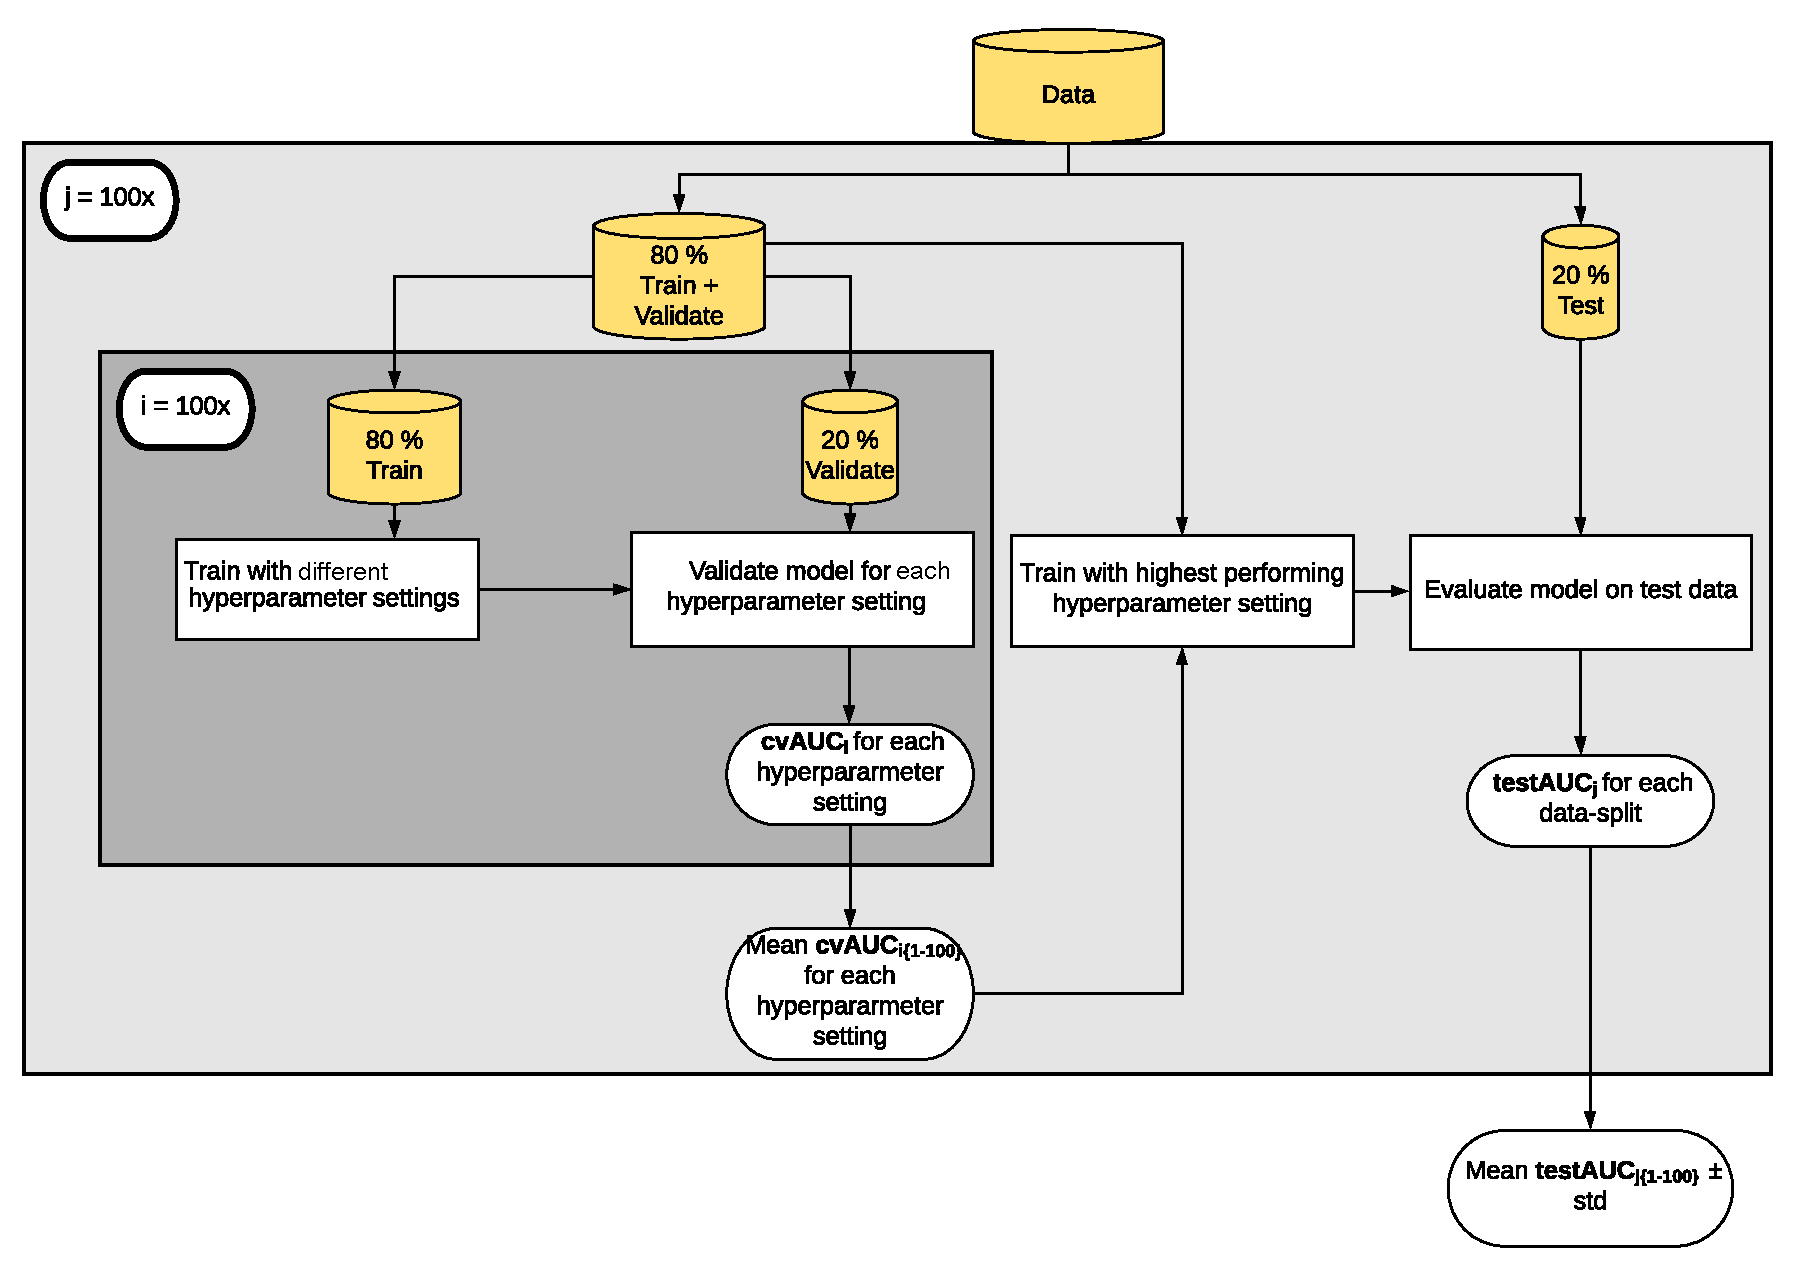
\includegraphics{Figure_1.pdf} \textbf{Figure 1. Machine learning
pipeline.} We split the data to create a training (80\%) and held-out
test set (20\%). The splits were stratified to maintain the overall
class distribution. We performed five-fold cross-validation on the
training data to select the best hyperparameter setting and then used
these hyperparameters to train the models. The model was evaluated on
the held-out data set. Abbreviations: cvAUC, cross-validation area under
the receiver operating characteristic curve. \newpage
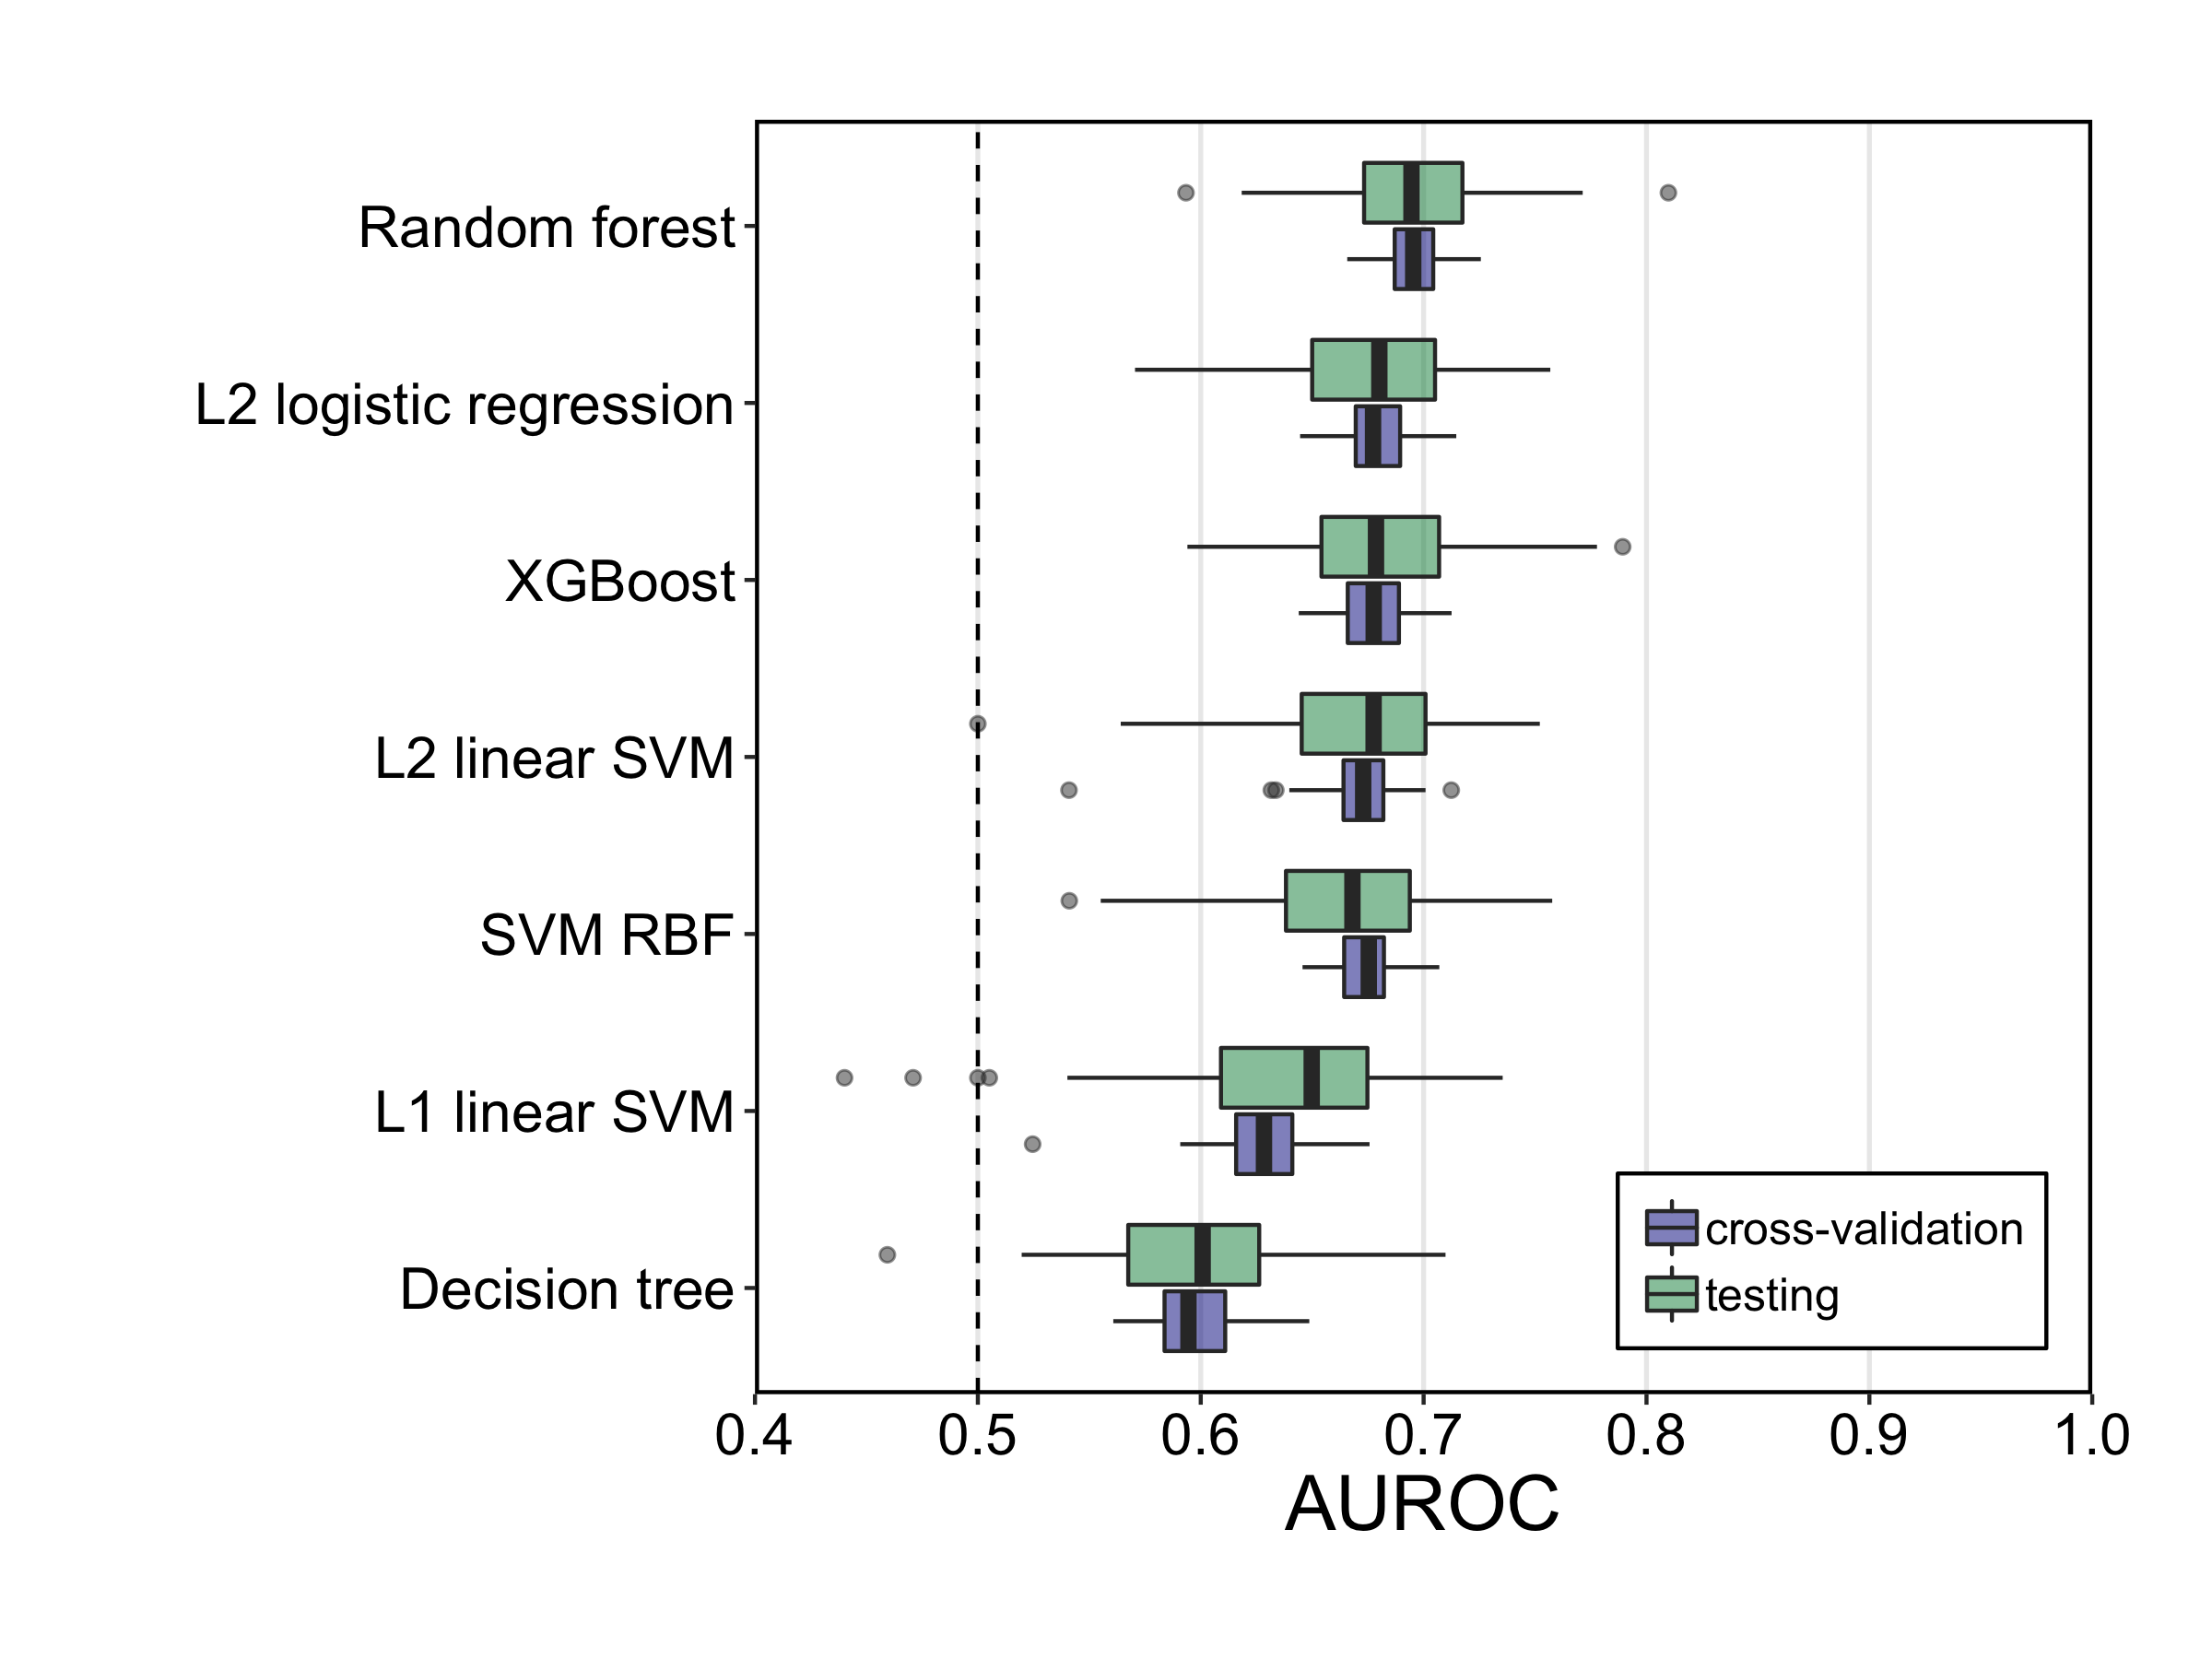
\includegraphics{Figure_2.png}

\textbf{Figure 2. Generalization and classification performance of ML
models using AUROC values of all cross validation and testing
performances.} The median AUROC for diagnosing individuals with SRN
using bacterial abundances was higher than chance (depicted by
horizontal line at 0.50) for all the ML models. The predictive
performance of random forest model was higher than other ML models,s
though not significantly (p=0.5). L2-regularized logistic regression,
XGBoost, L2-regularized SVM with linear and radial basis function kernel
performances were not significantly different from one another. The
boxplot shows quartiles at the box ends and the median as the horizontal
line in the box. The whiskers show the farthest points that were not
outliers. Outliers were defined as those data points that are not within
1.5 times the interquartile ranges. \newpage
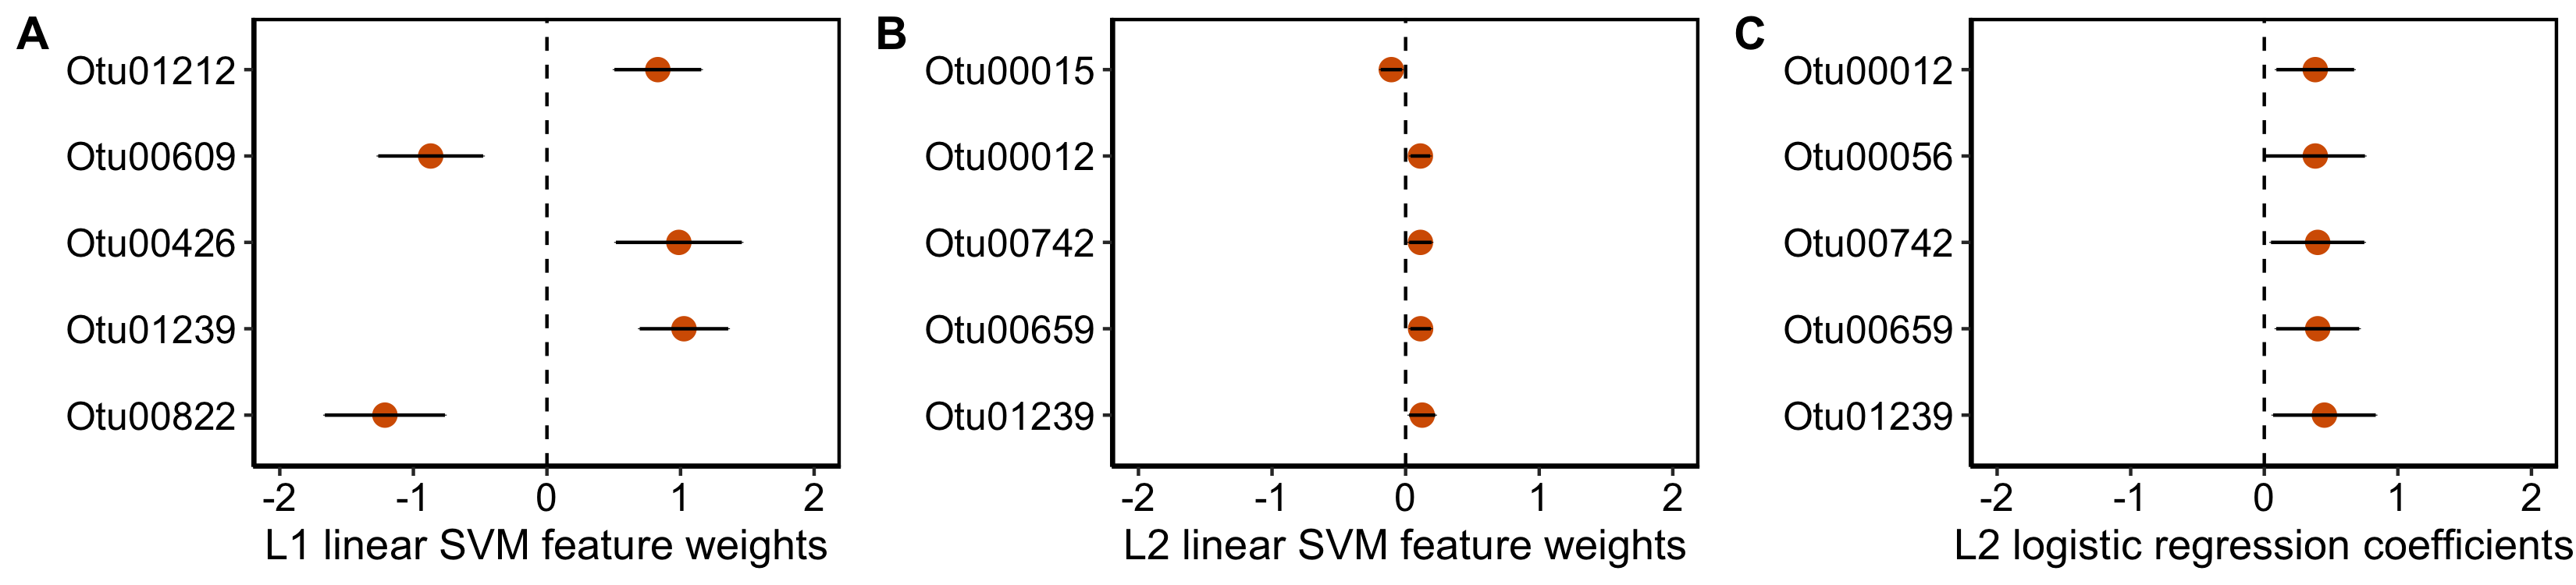
\includegraphics[height=17cm, width=12cm]{Figure_3.png}

\textbf{Figure 3. Interpretation of the linear ML models.} The ranks of
absolute feature weights of (A) L1-regularized SVM with linear kernel,
(B) L2-regularized SVM with linear kernel, and (C) L2-regularized
logistic regression, were ranked from highest rank, 1, to lowest rank,
100, for each datasplit. The feature ranks of the 20 highest ranked OTUs
based on their median ranks (median shown in black) are reported here.
OTUs that were associated with classifying a subject as being healthy
had negative signs and were shown in blue. OTUs that were associated
with classifying a subject having an SRN had positive signs and were
shown in red. Some of the same OTUs were identified as important in all
of the linear models. \newpage
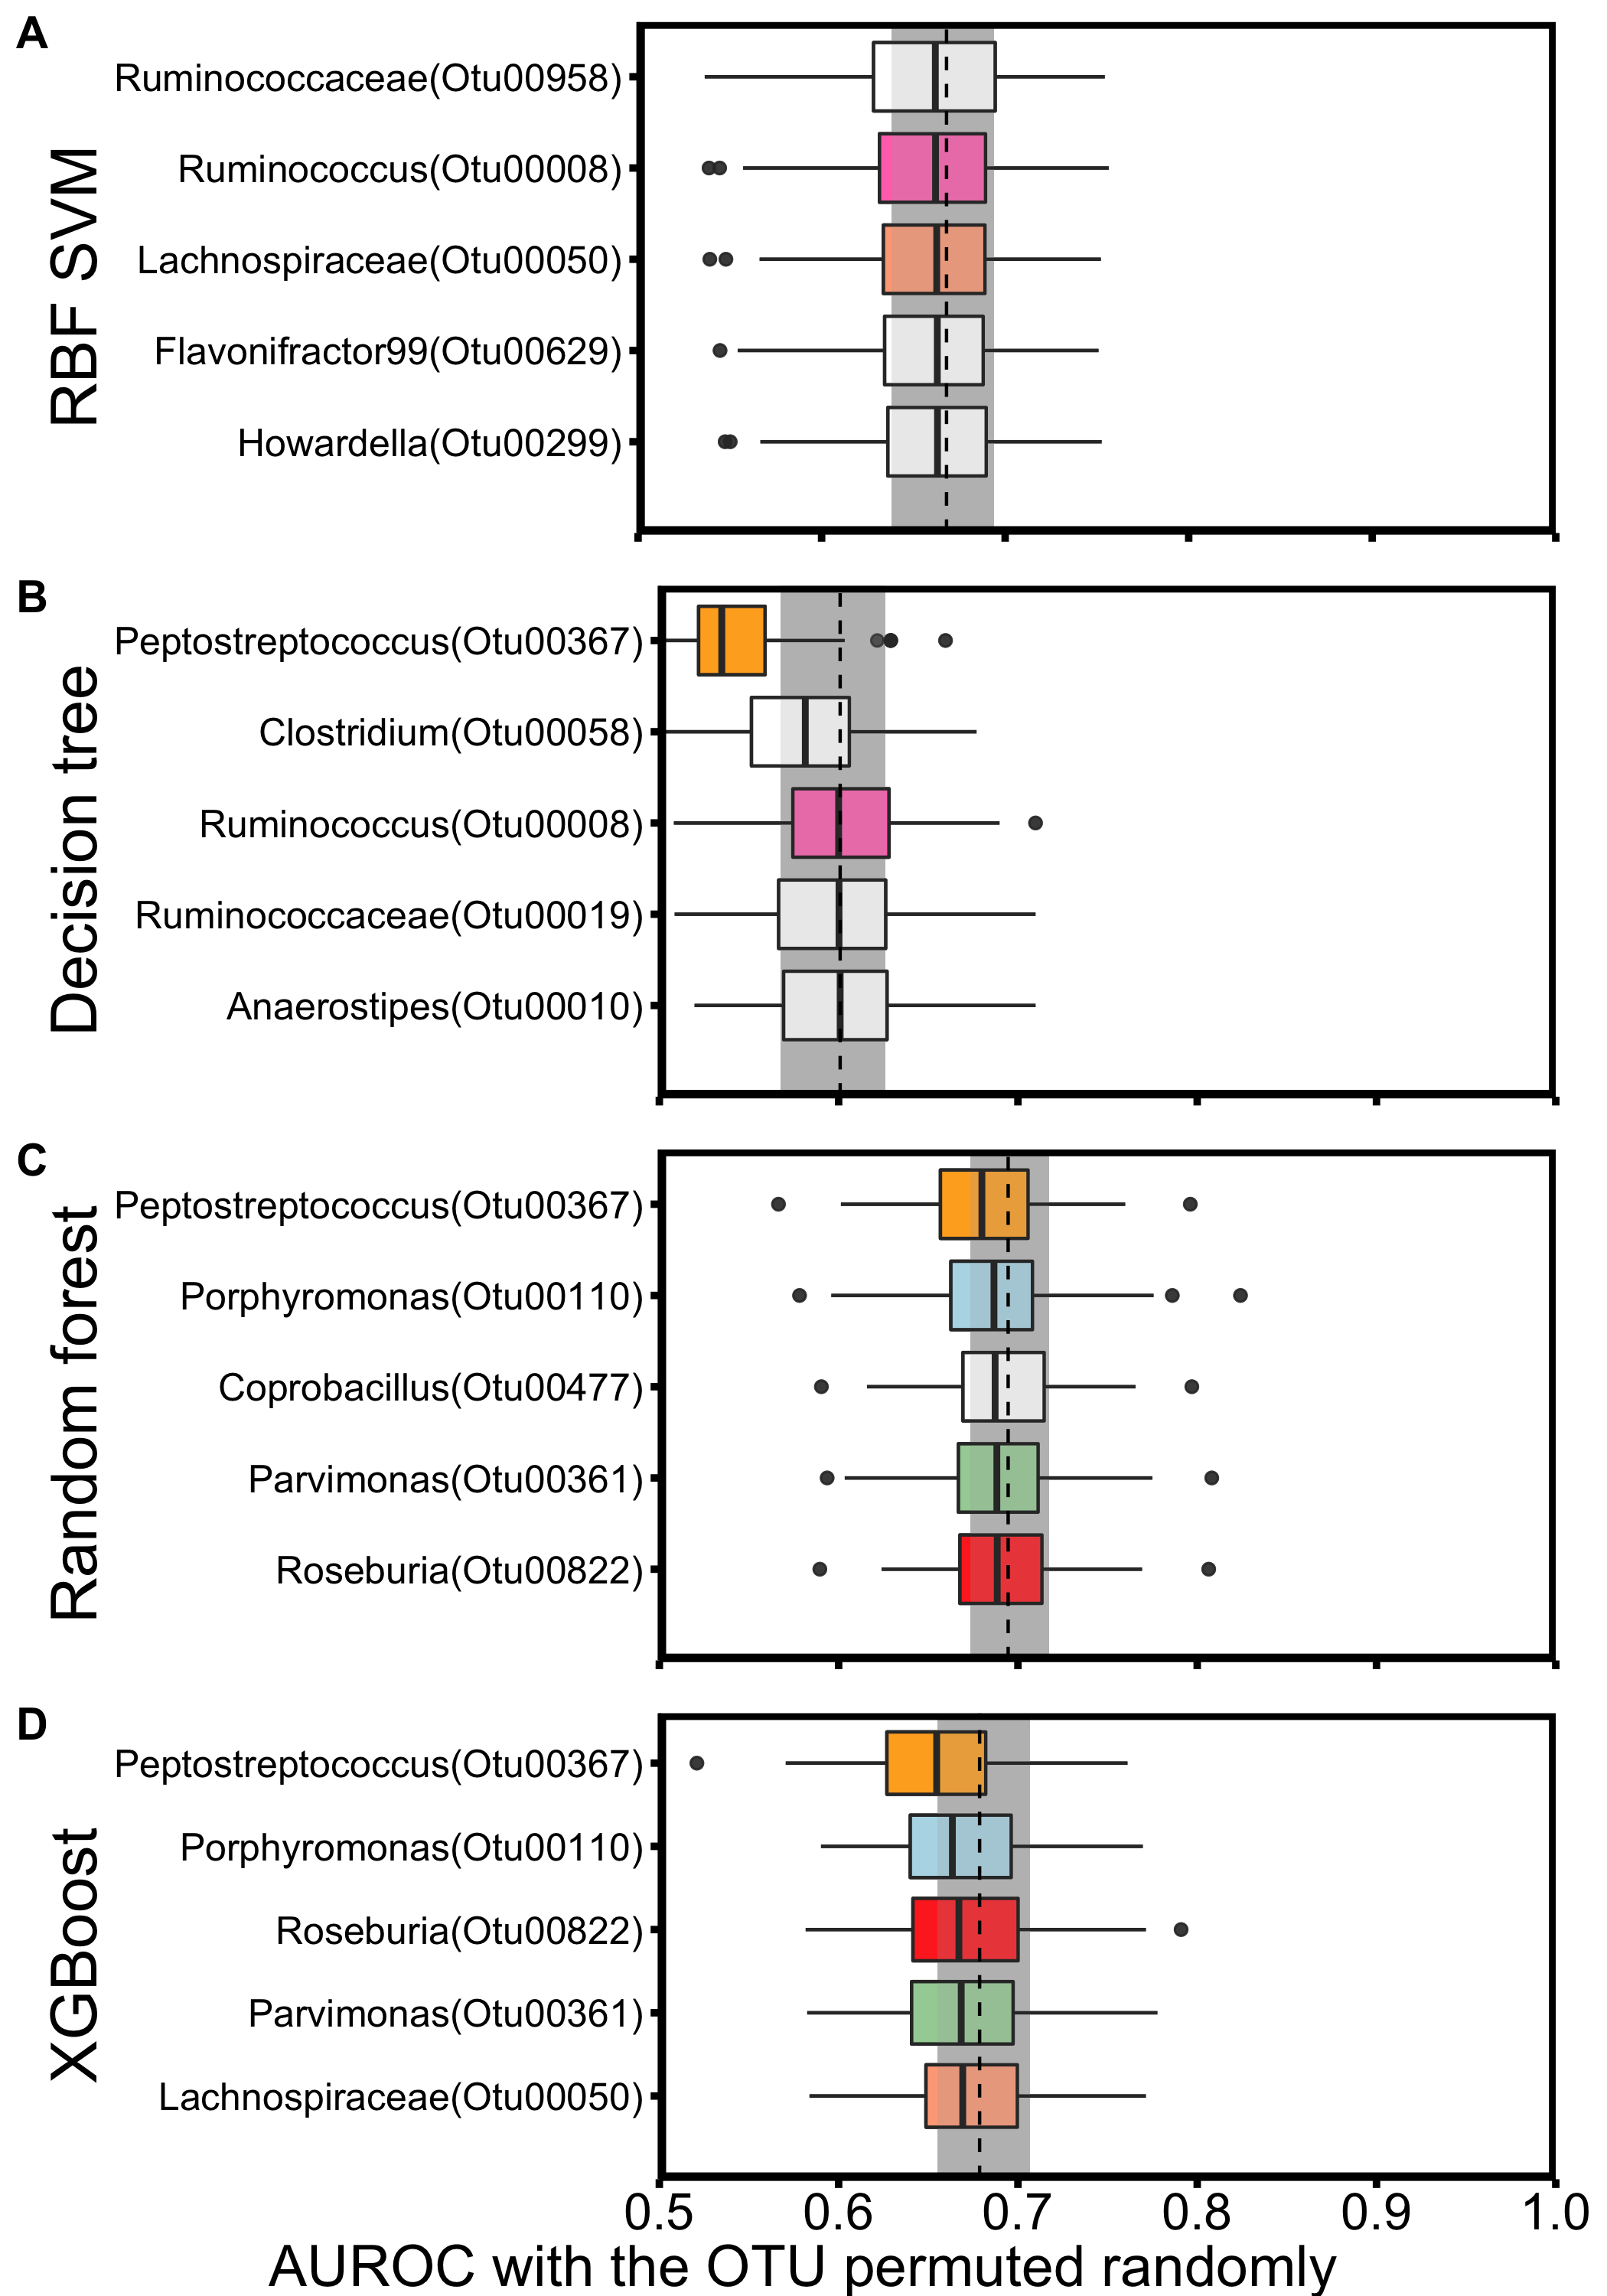
\includegraphics{Figure_4.png}

\textbf{Figure 4. Interpretation of the non-linear ML models.} (A) SVM
with radial basis kernel, (B) decision tree, (C) random forest, and (D)
XGBoost feature importances were explained using permutation importance
on the held-out test data set. The gray rectangle and the dashed line
show the IQR range and median of the base testing AUROC without any
permutation. The 20 OTUs that caused the largest decrease in the AUROC
when permuted are reported here. The colors of the box plots represent
the OTUs that were shared among the different models; yellow were OTUs
that were shared among all the non-linear models, salmon were OTUs that
were shared among the tree-based models, green were the OTUs shared
among SVM with radial basis kernel, decision tree and XGBoost, pink were
the OTUs shared among SVM with radial basis kernel and XGBoost only, red
were the OTUs shared among random forest and XGBoost only and blue were
the OTUs shared among decision tree and random forest only. For all of
the tree-based models, a \emph{Peptostreptococcus} species (OTU00367)
had the largest impact on predictive performance. \newpage
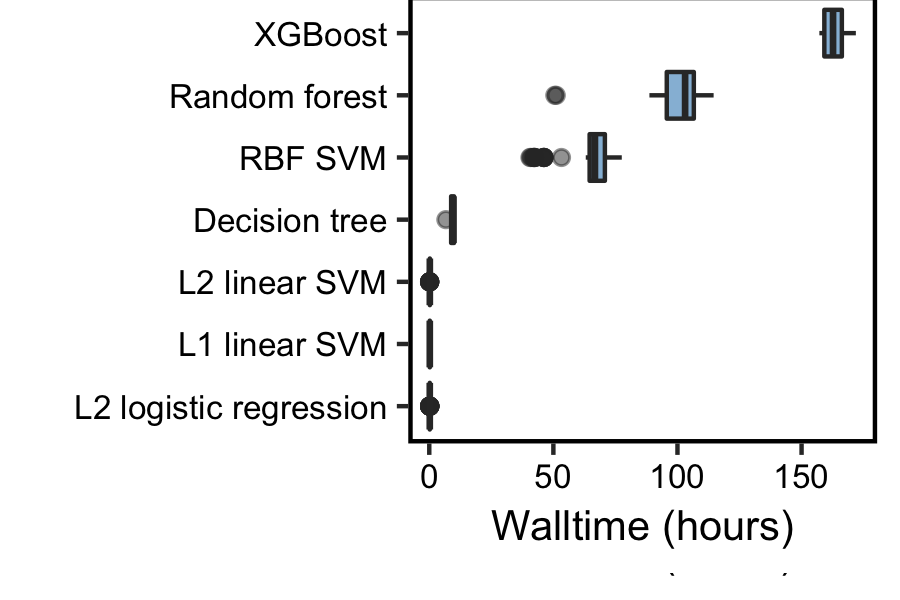
\includegraphics{Figure_5.png}

\textbf{Figure 5. Training times of seven ML models.} The median
training time was the highest for XGBoost and shortest for
L2-regularized logistic regression. \newpage
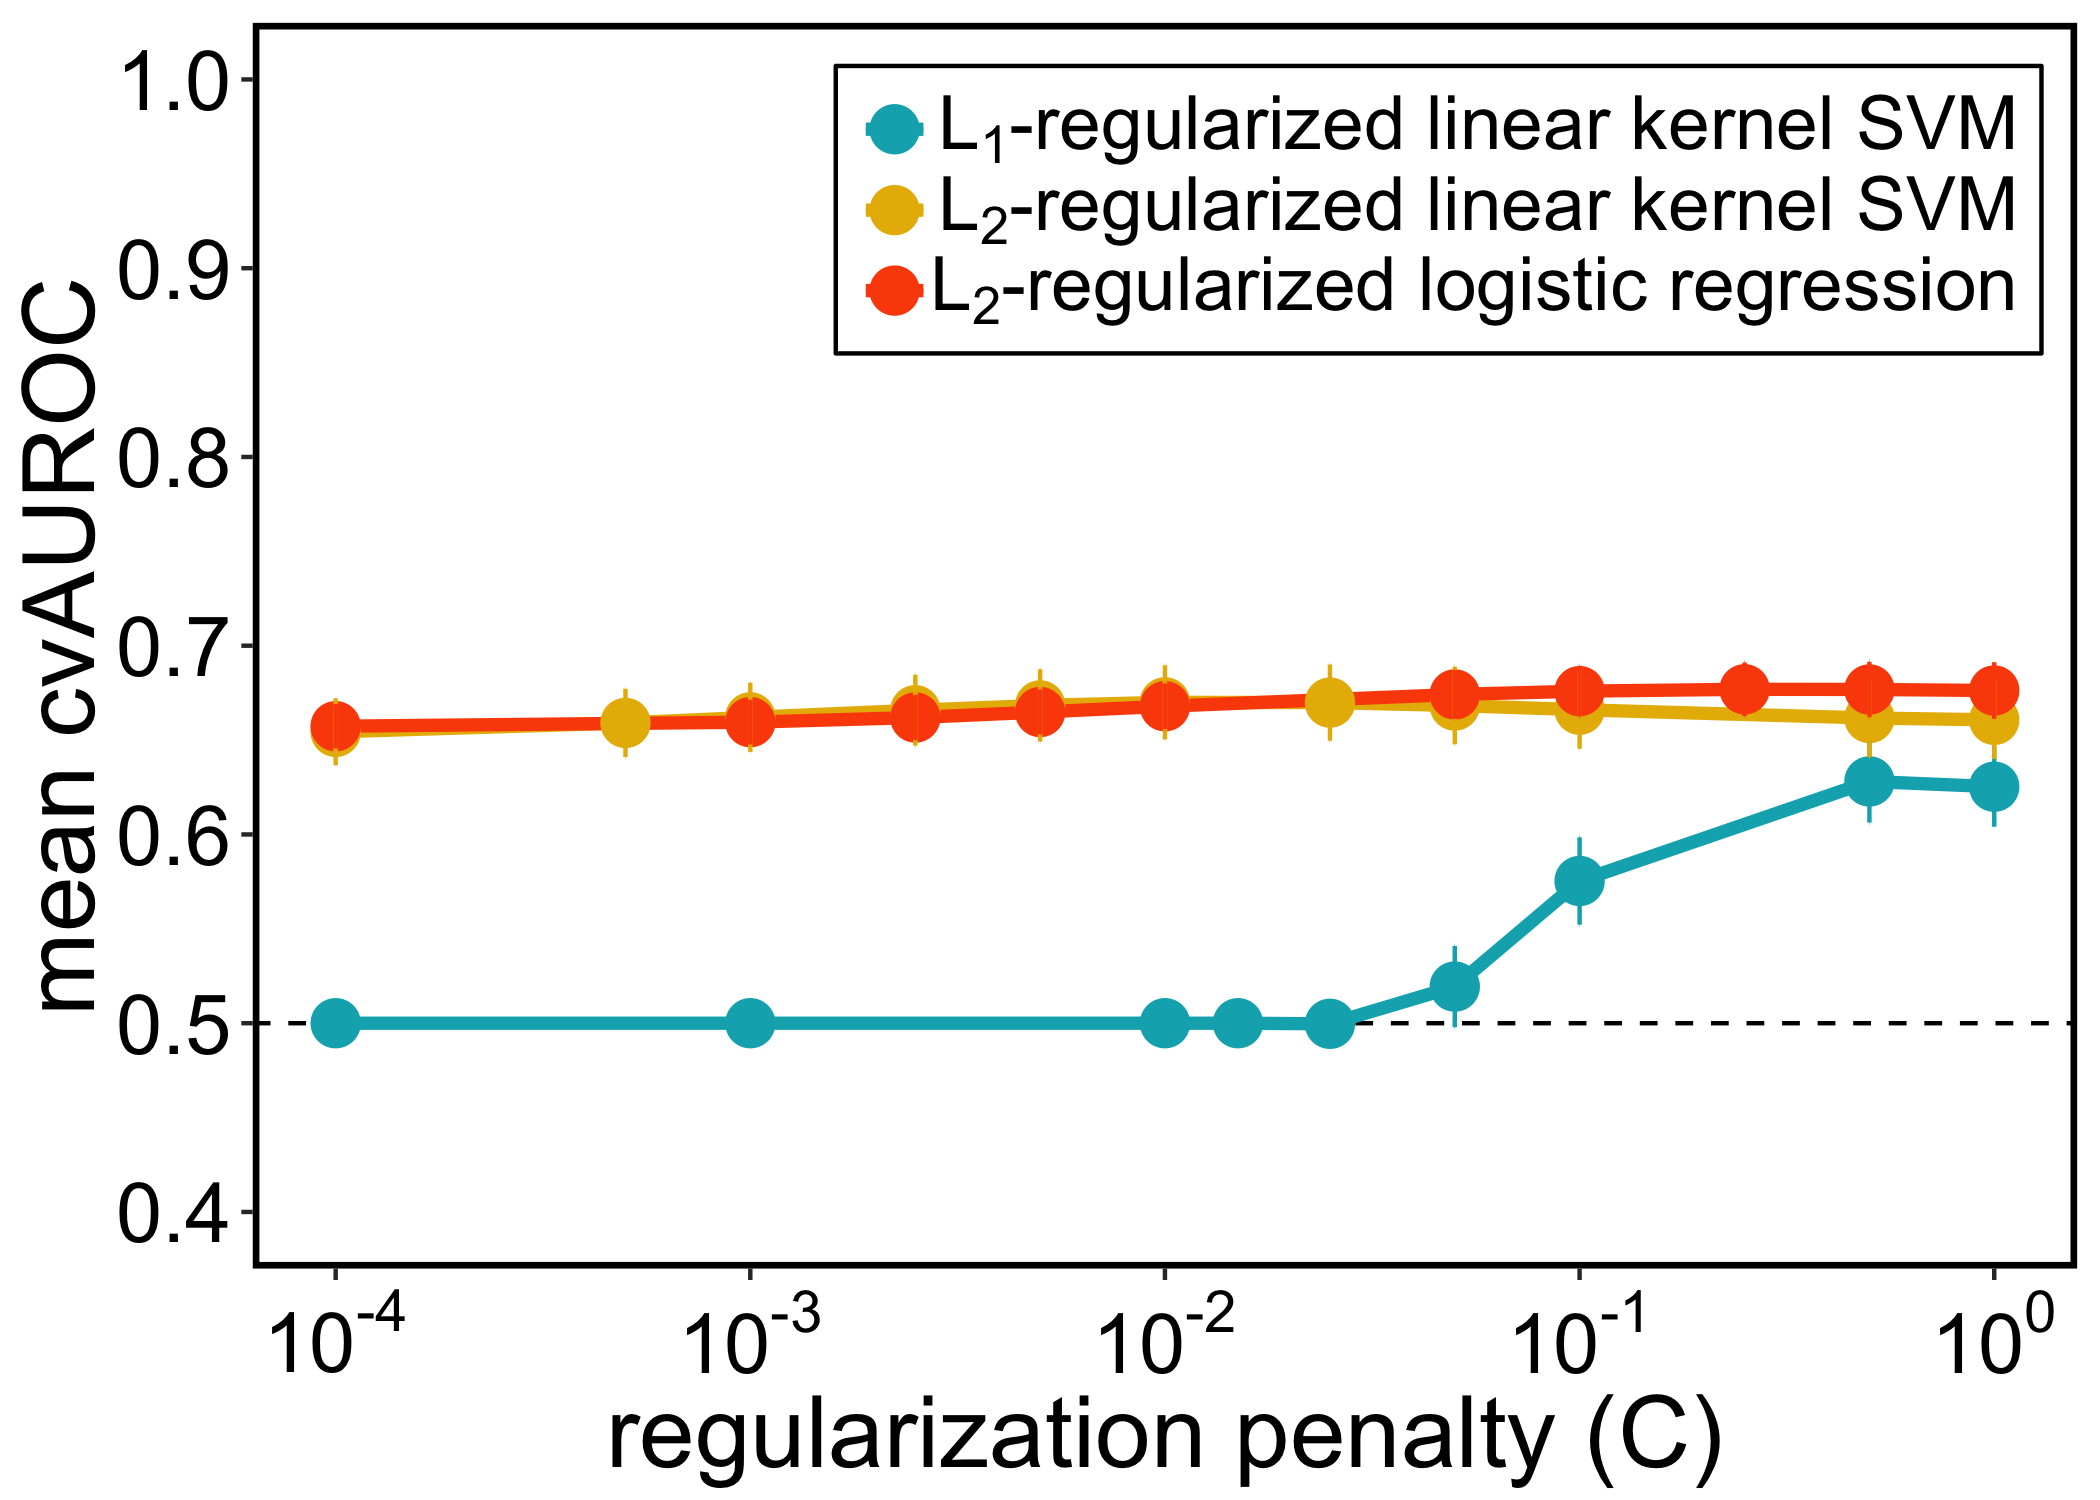
\includegraphics{Figure_S1.png}

\textbf{Figure S1. Hyperparameter setting performances for linear
models.} (A) L2-regularized logistic regression, (B) L1-regularized SVM
with linear kernel, and (C) L2-regularized SVM with linear kernel mean
cross-validation AUROC values when different hyperparameters were used
in training the model. The stars represent the highest performing
hyperparameter setting for each model. \newpage
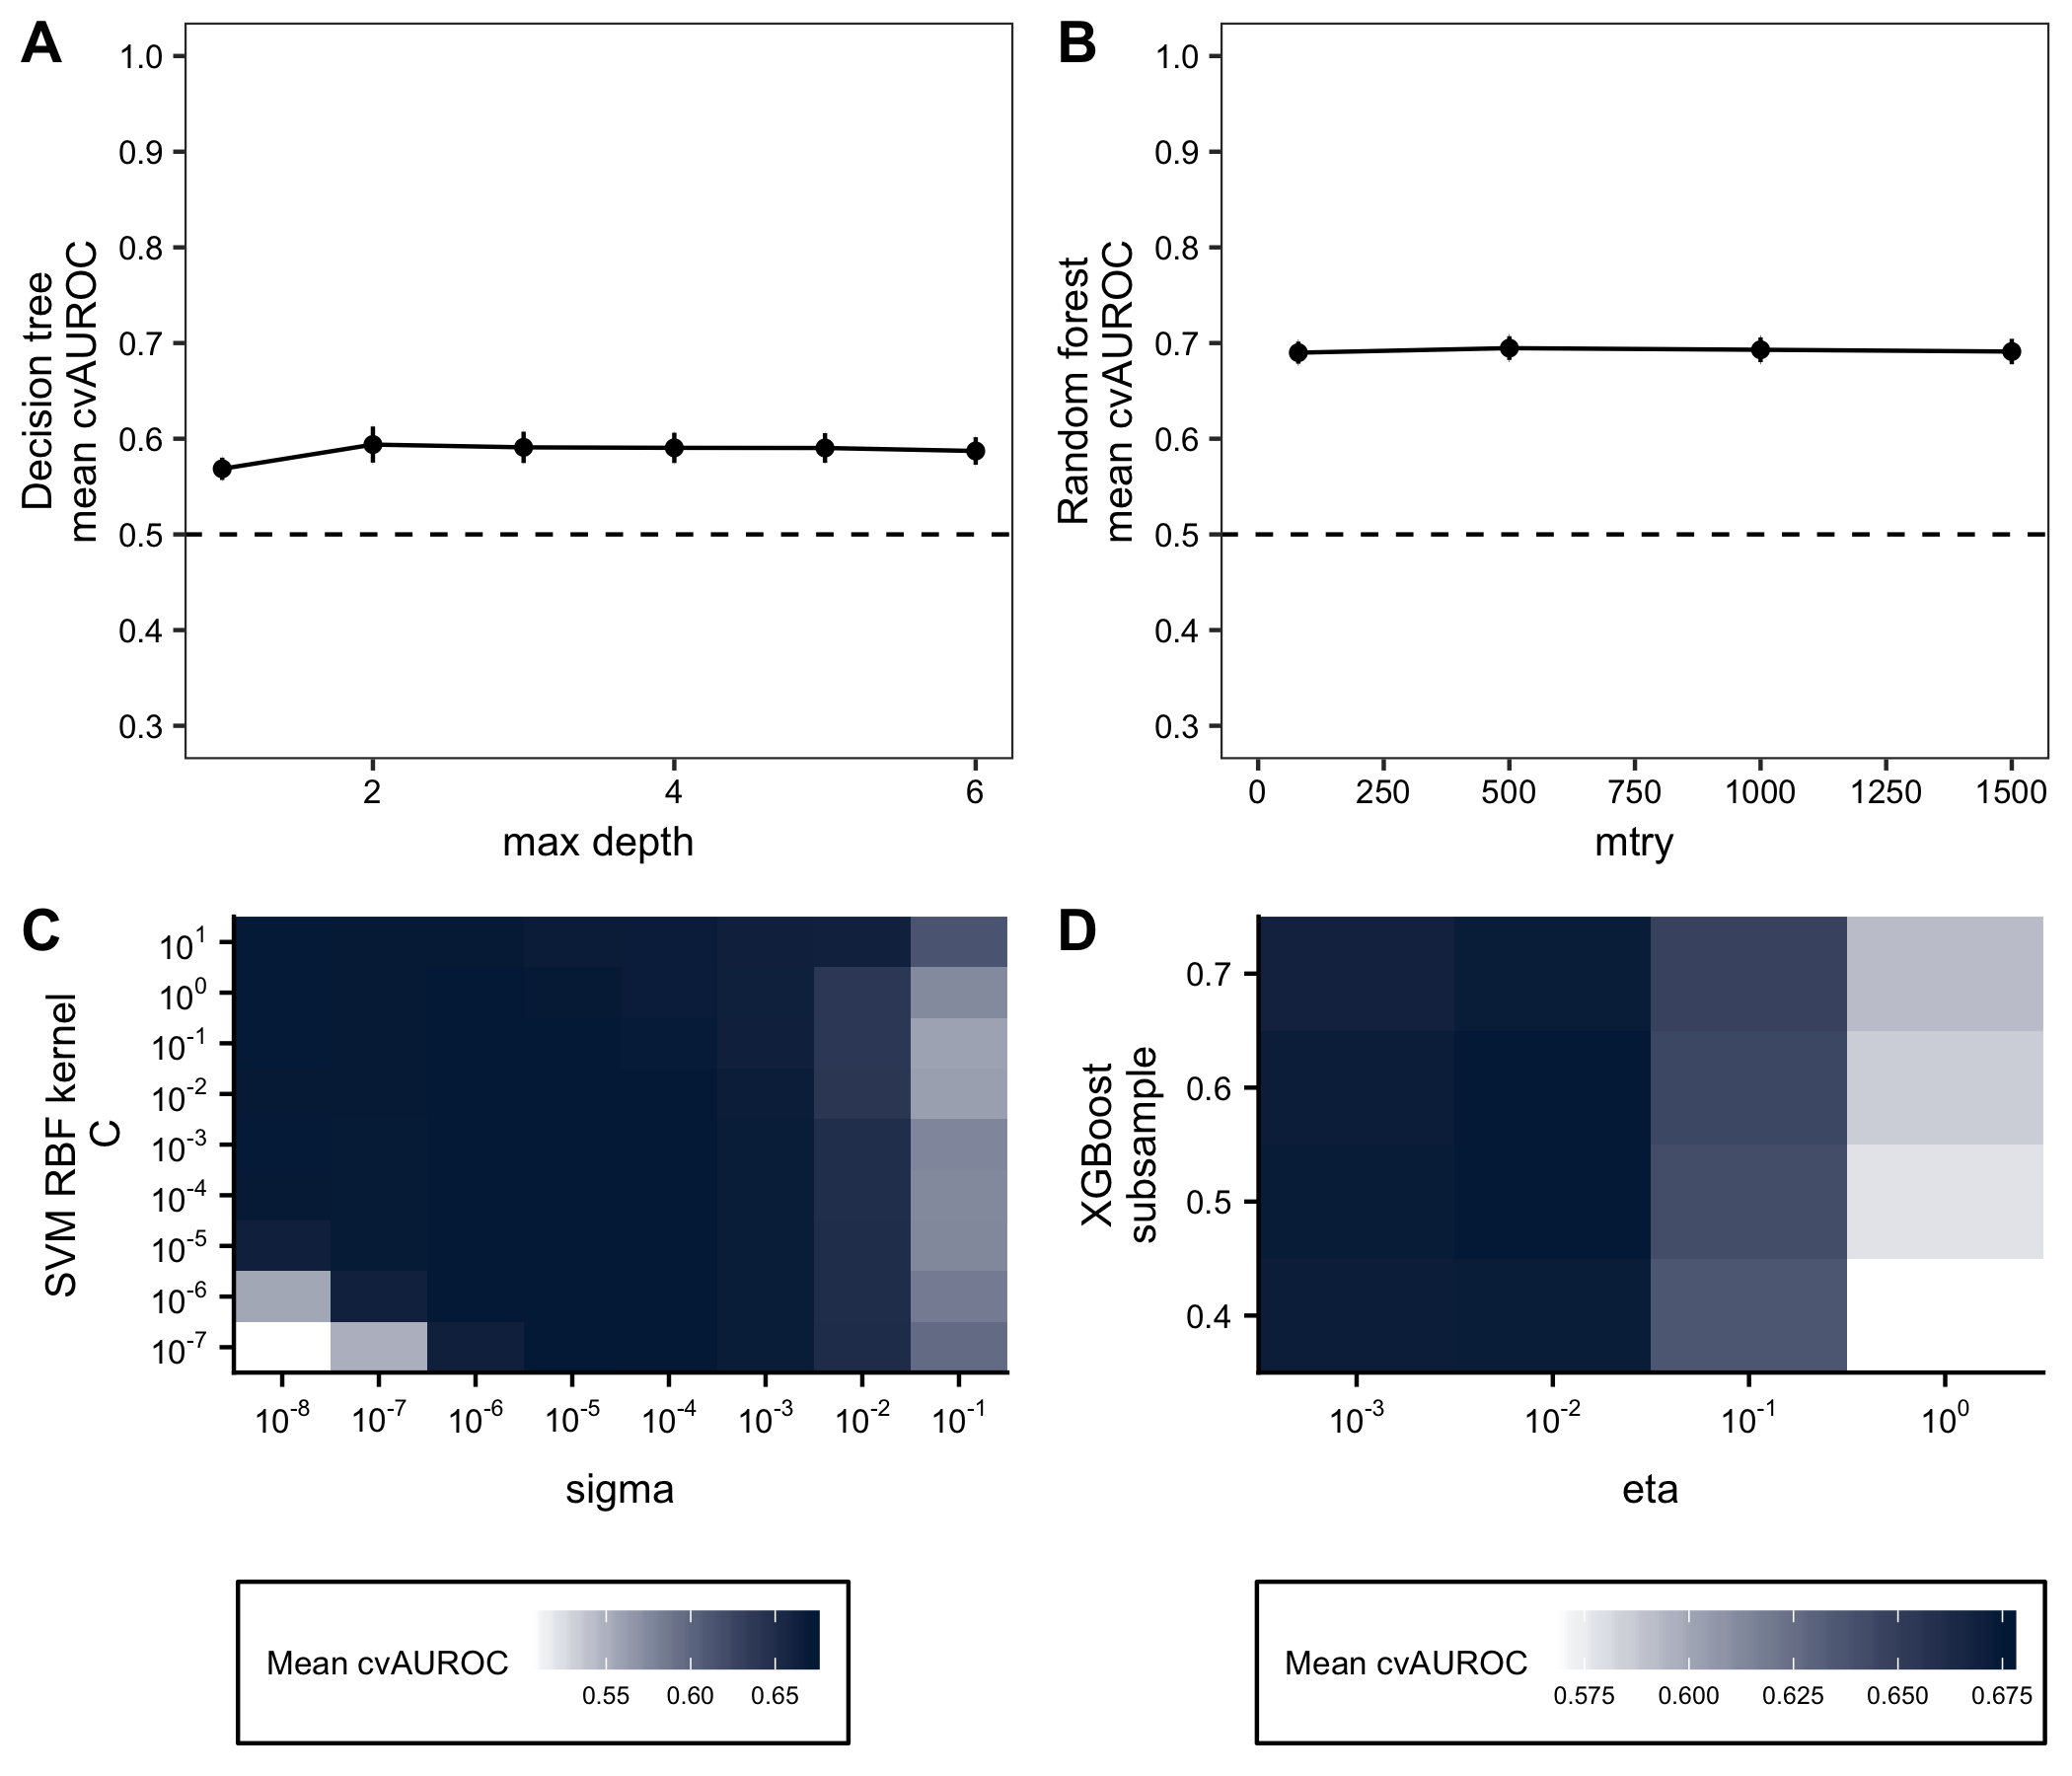
\includegraphics[height=30cm, width=15cm]{Figure_S2.png}

\textbf{Figure S2. Hyperparameter setting performances for non-linear
models.} (A) Decision tree, (B) random forest, (C) SVM with radial basis
kernel, and (D) XGBoost mean cross-validation AUROC values when
different hyperparameters were used in training the model. The stars
represent the highest performing hyperparameter setting for the models.
\newpage
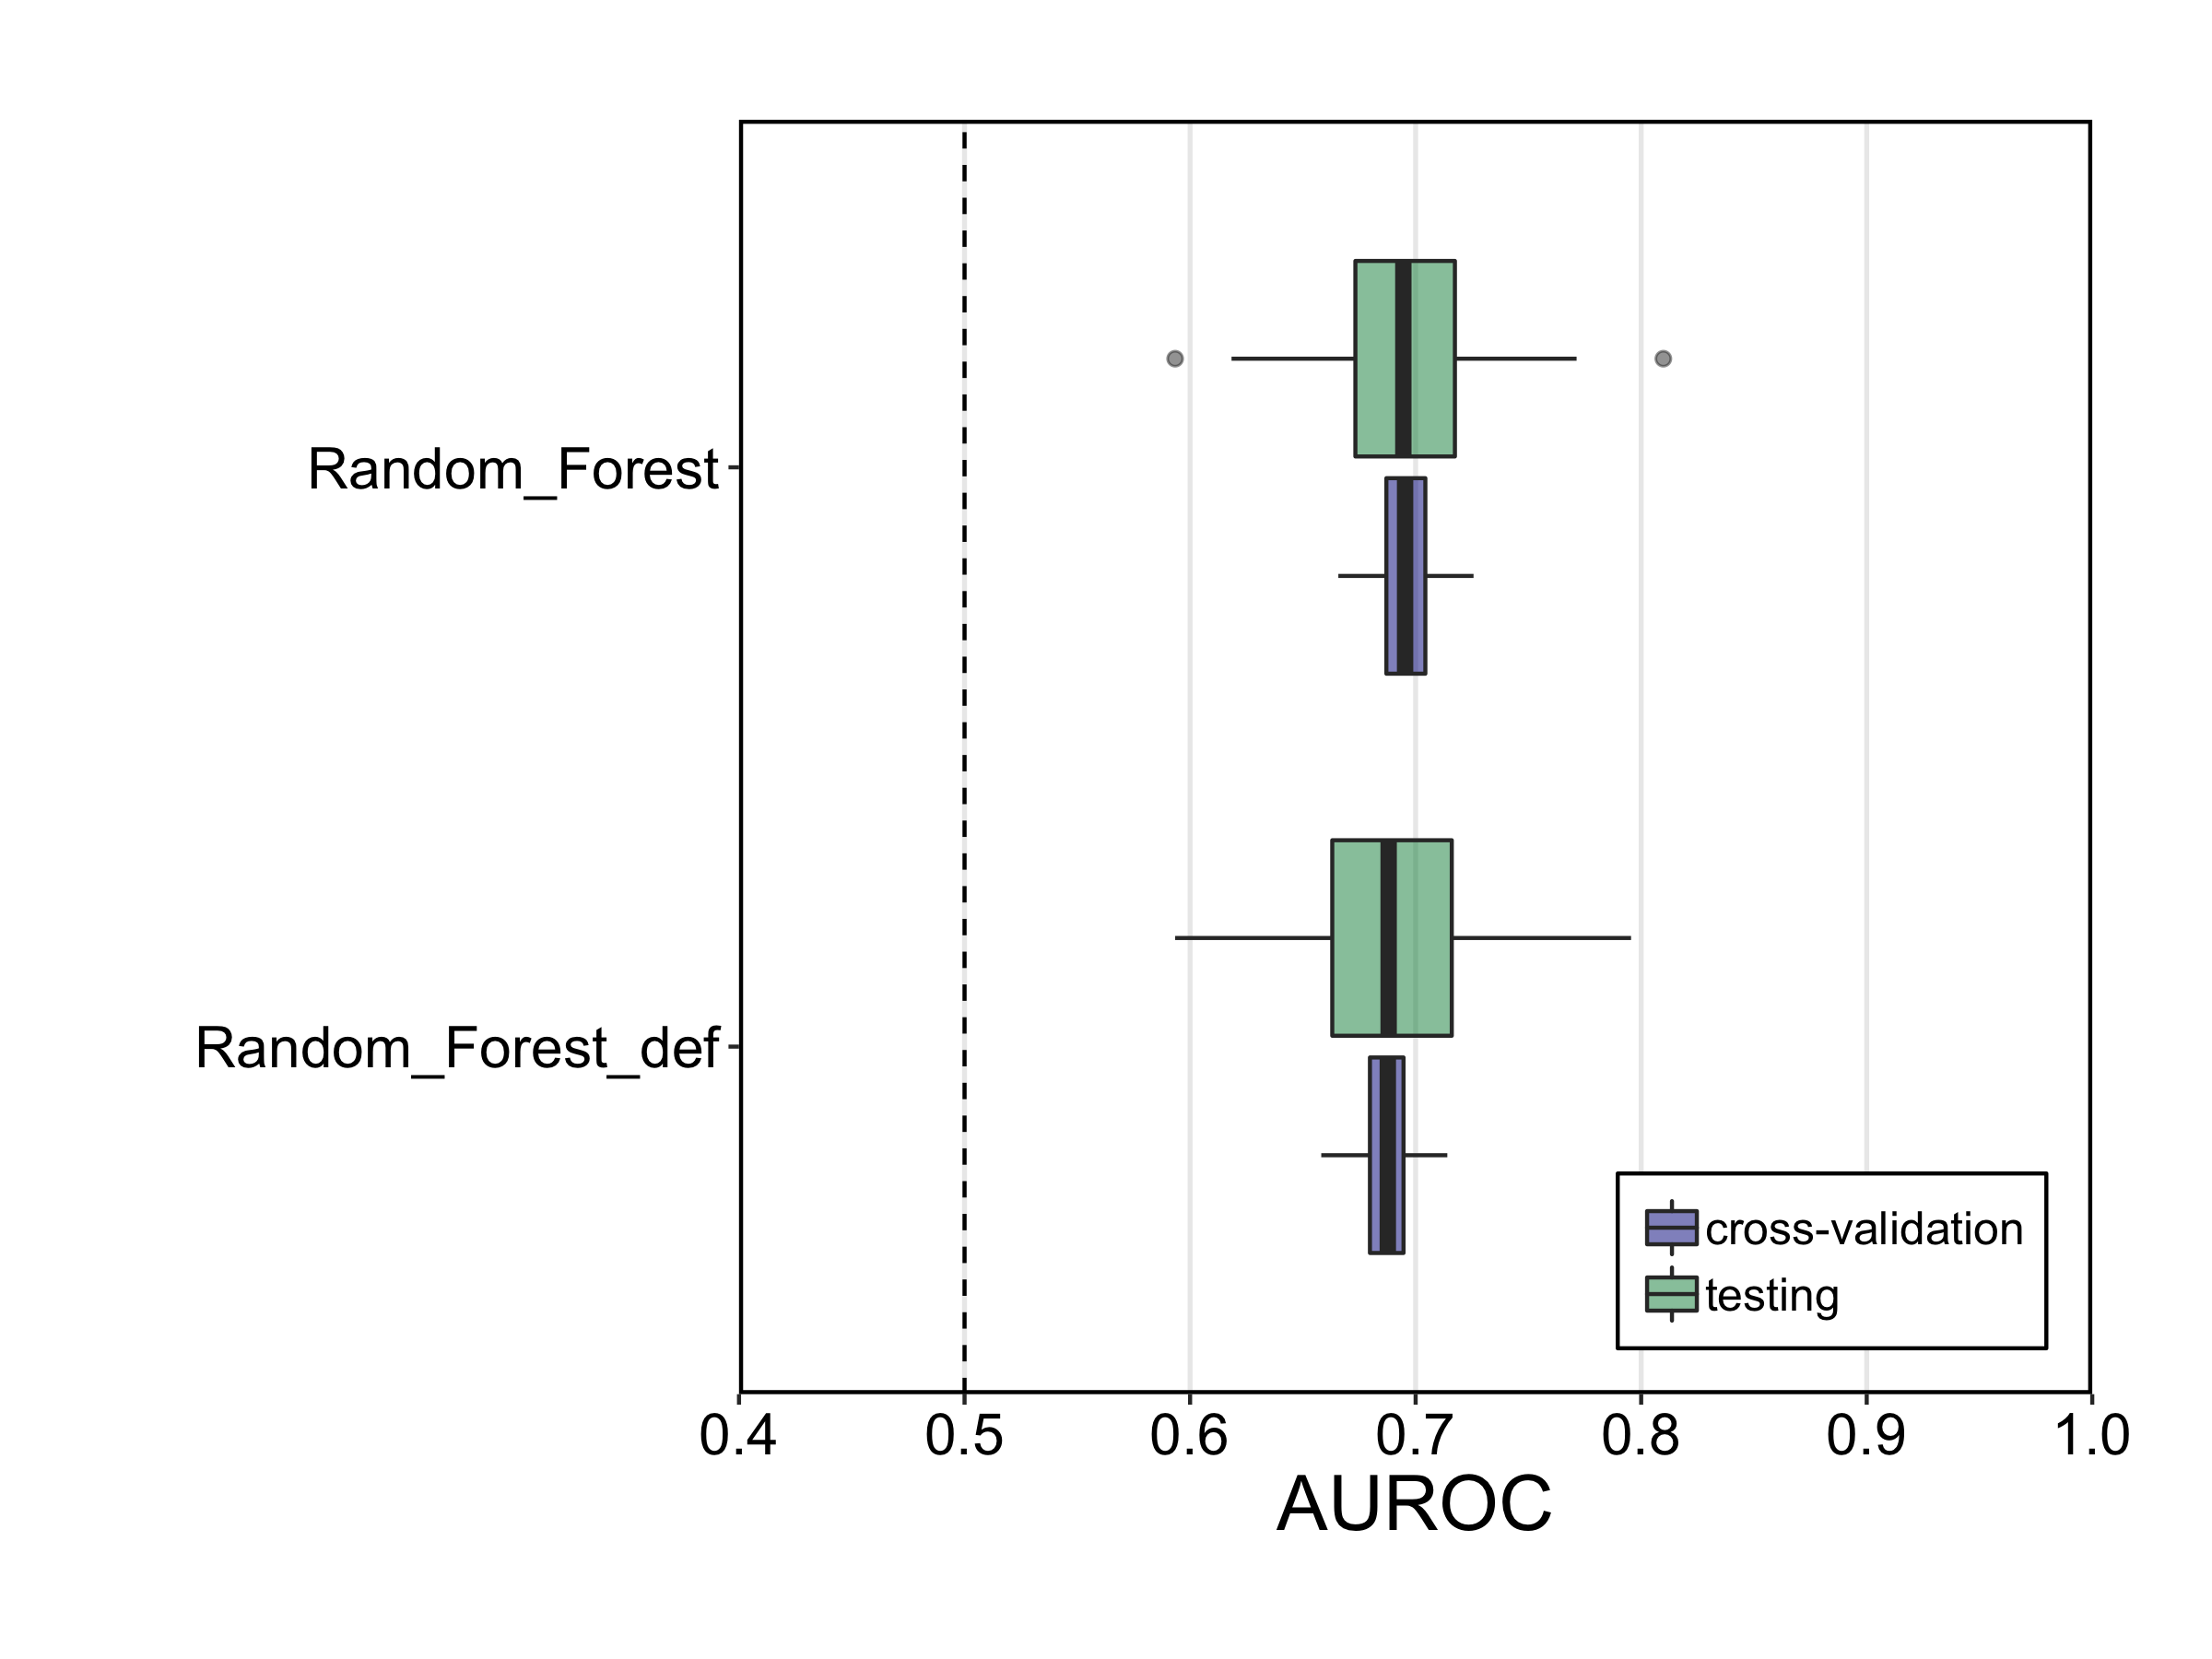
\includegraphics[height=17.5cm, width=13cm]{Figure_S3.png}

\textbf{Figure S3. Histogram of AUROC differences between L2-regularized
logistic regression and random forest for each of the hundred
datasplits.} This histogram shows number of datasplits in each bin. The
percentage of dataplits where the difference between random forest and
L2-regularized logistic regression AUROC values was higher than or equal
to 0 were 0.75, lower than or equal to 0 were 0.25. The vertical red
line highlights the bins where there AUROC difference between the two
model is 0. The p-value was calculated for a double tail event. \newpage
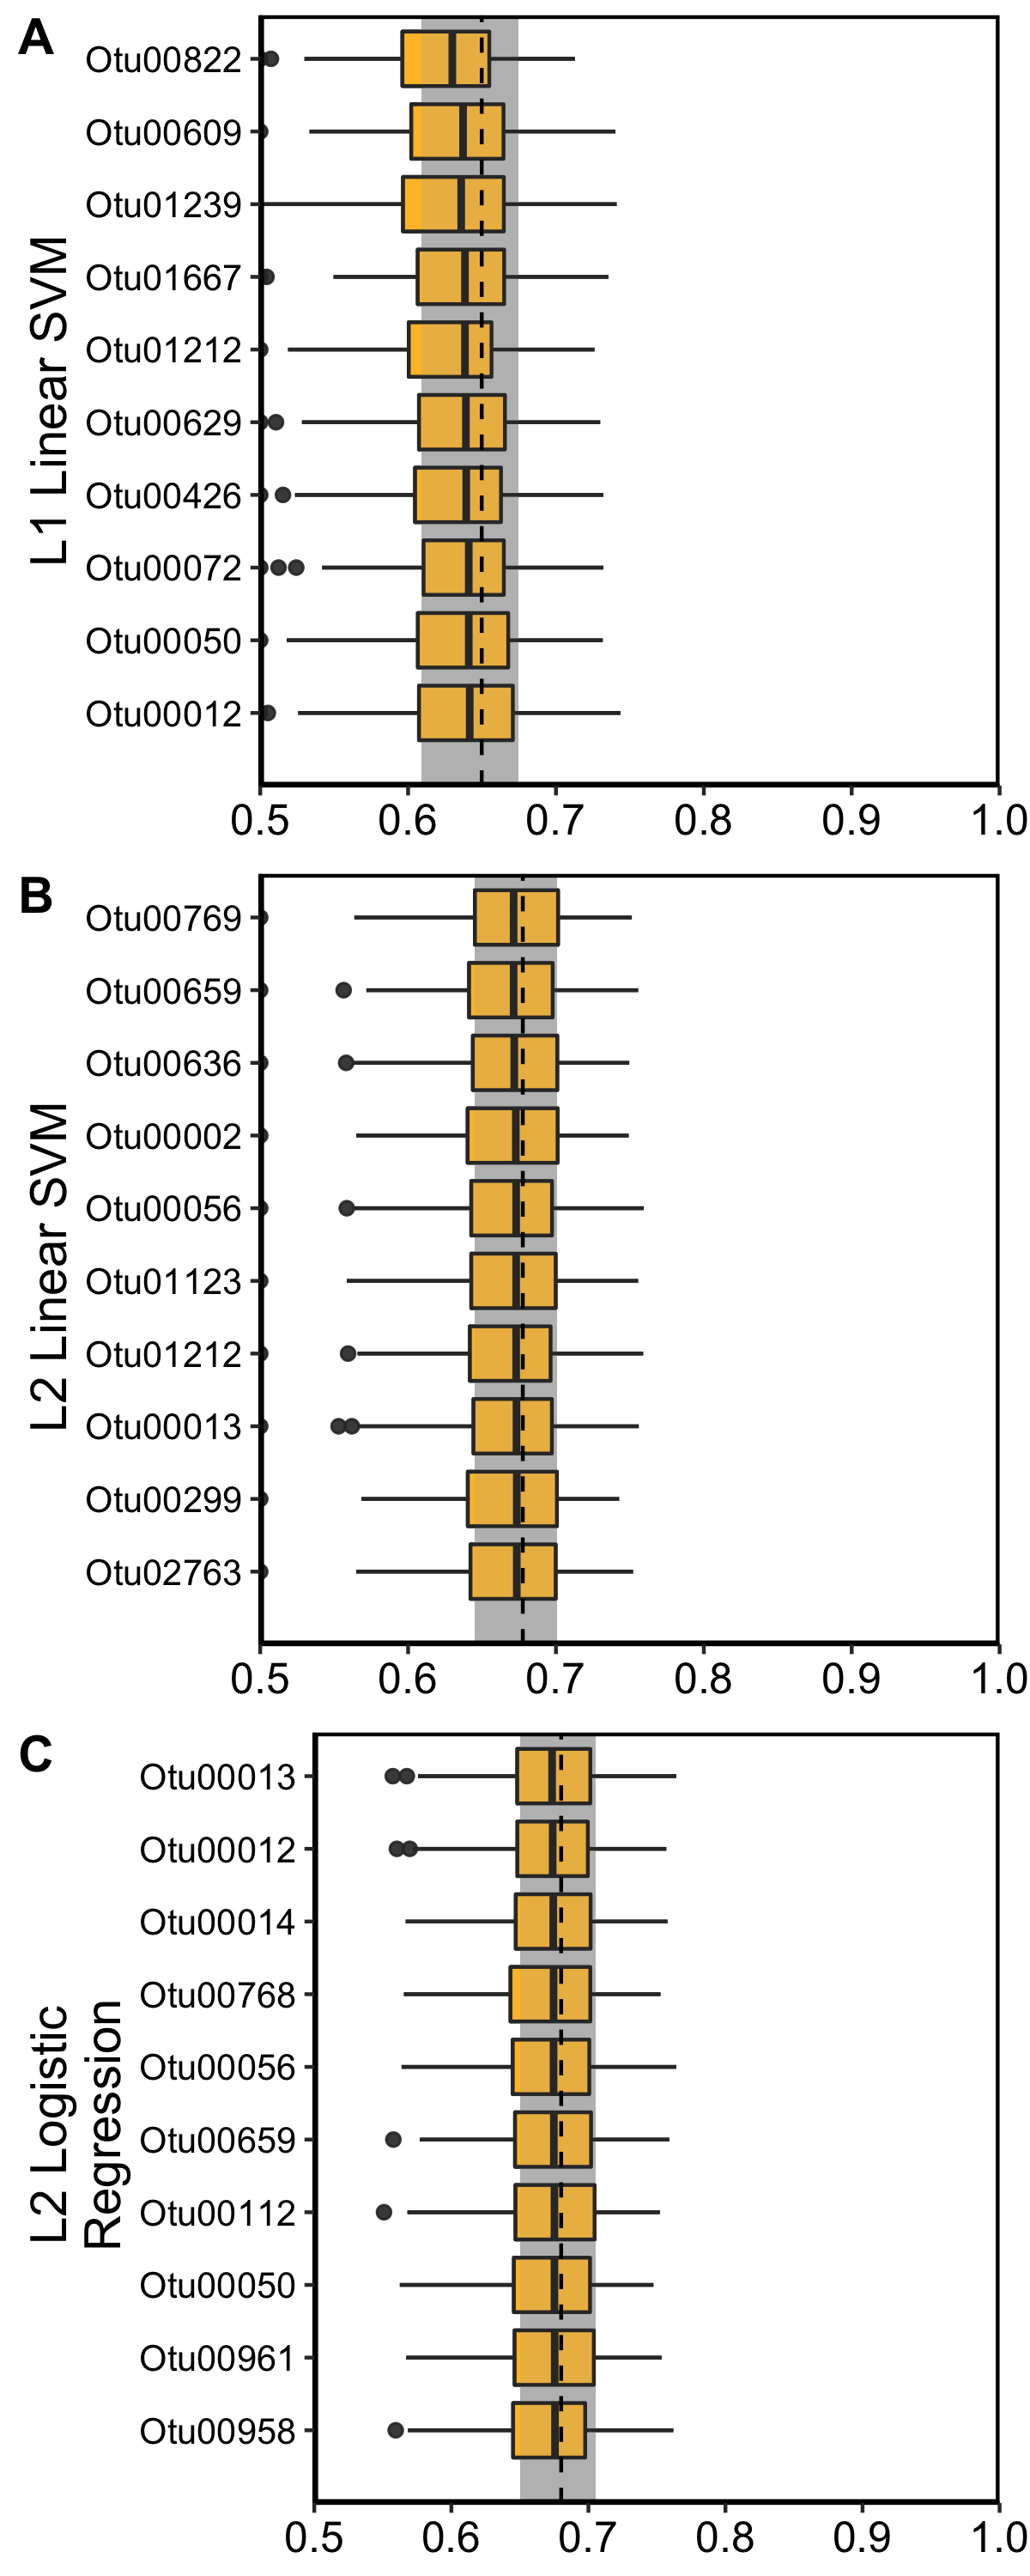
\includegraphics[height=17.5cm, width=13cm]{Figure_S4.png}

\textbf{Figure S4. Classification performance of ML models across cross
validation when trained on a subset of the dataset.} (A) L2-regularized
logistic regression and (B) random forest models were trained using the
original study design with 490 subjects and subsets of it with 15, 30,
60, 120, and 245 subjects. The range among the cross-validation AUROC
values within both models at lower sample sizes were much larger than
when the full collection of samples was used to train and validate the
models, but included the ranges observed with the more complete
datasets. \newpage
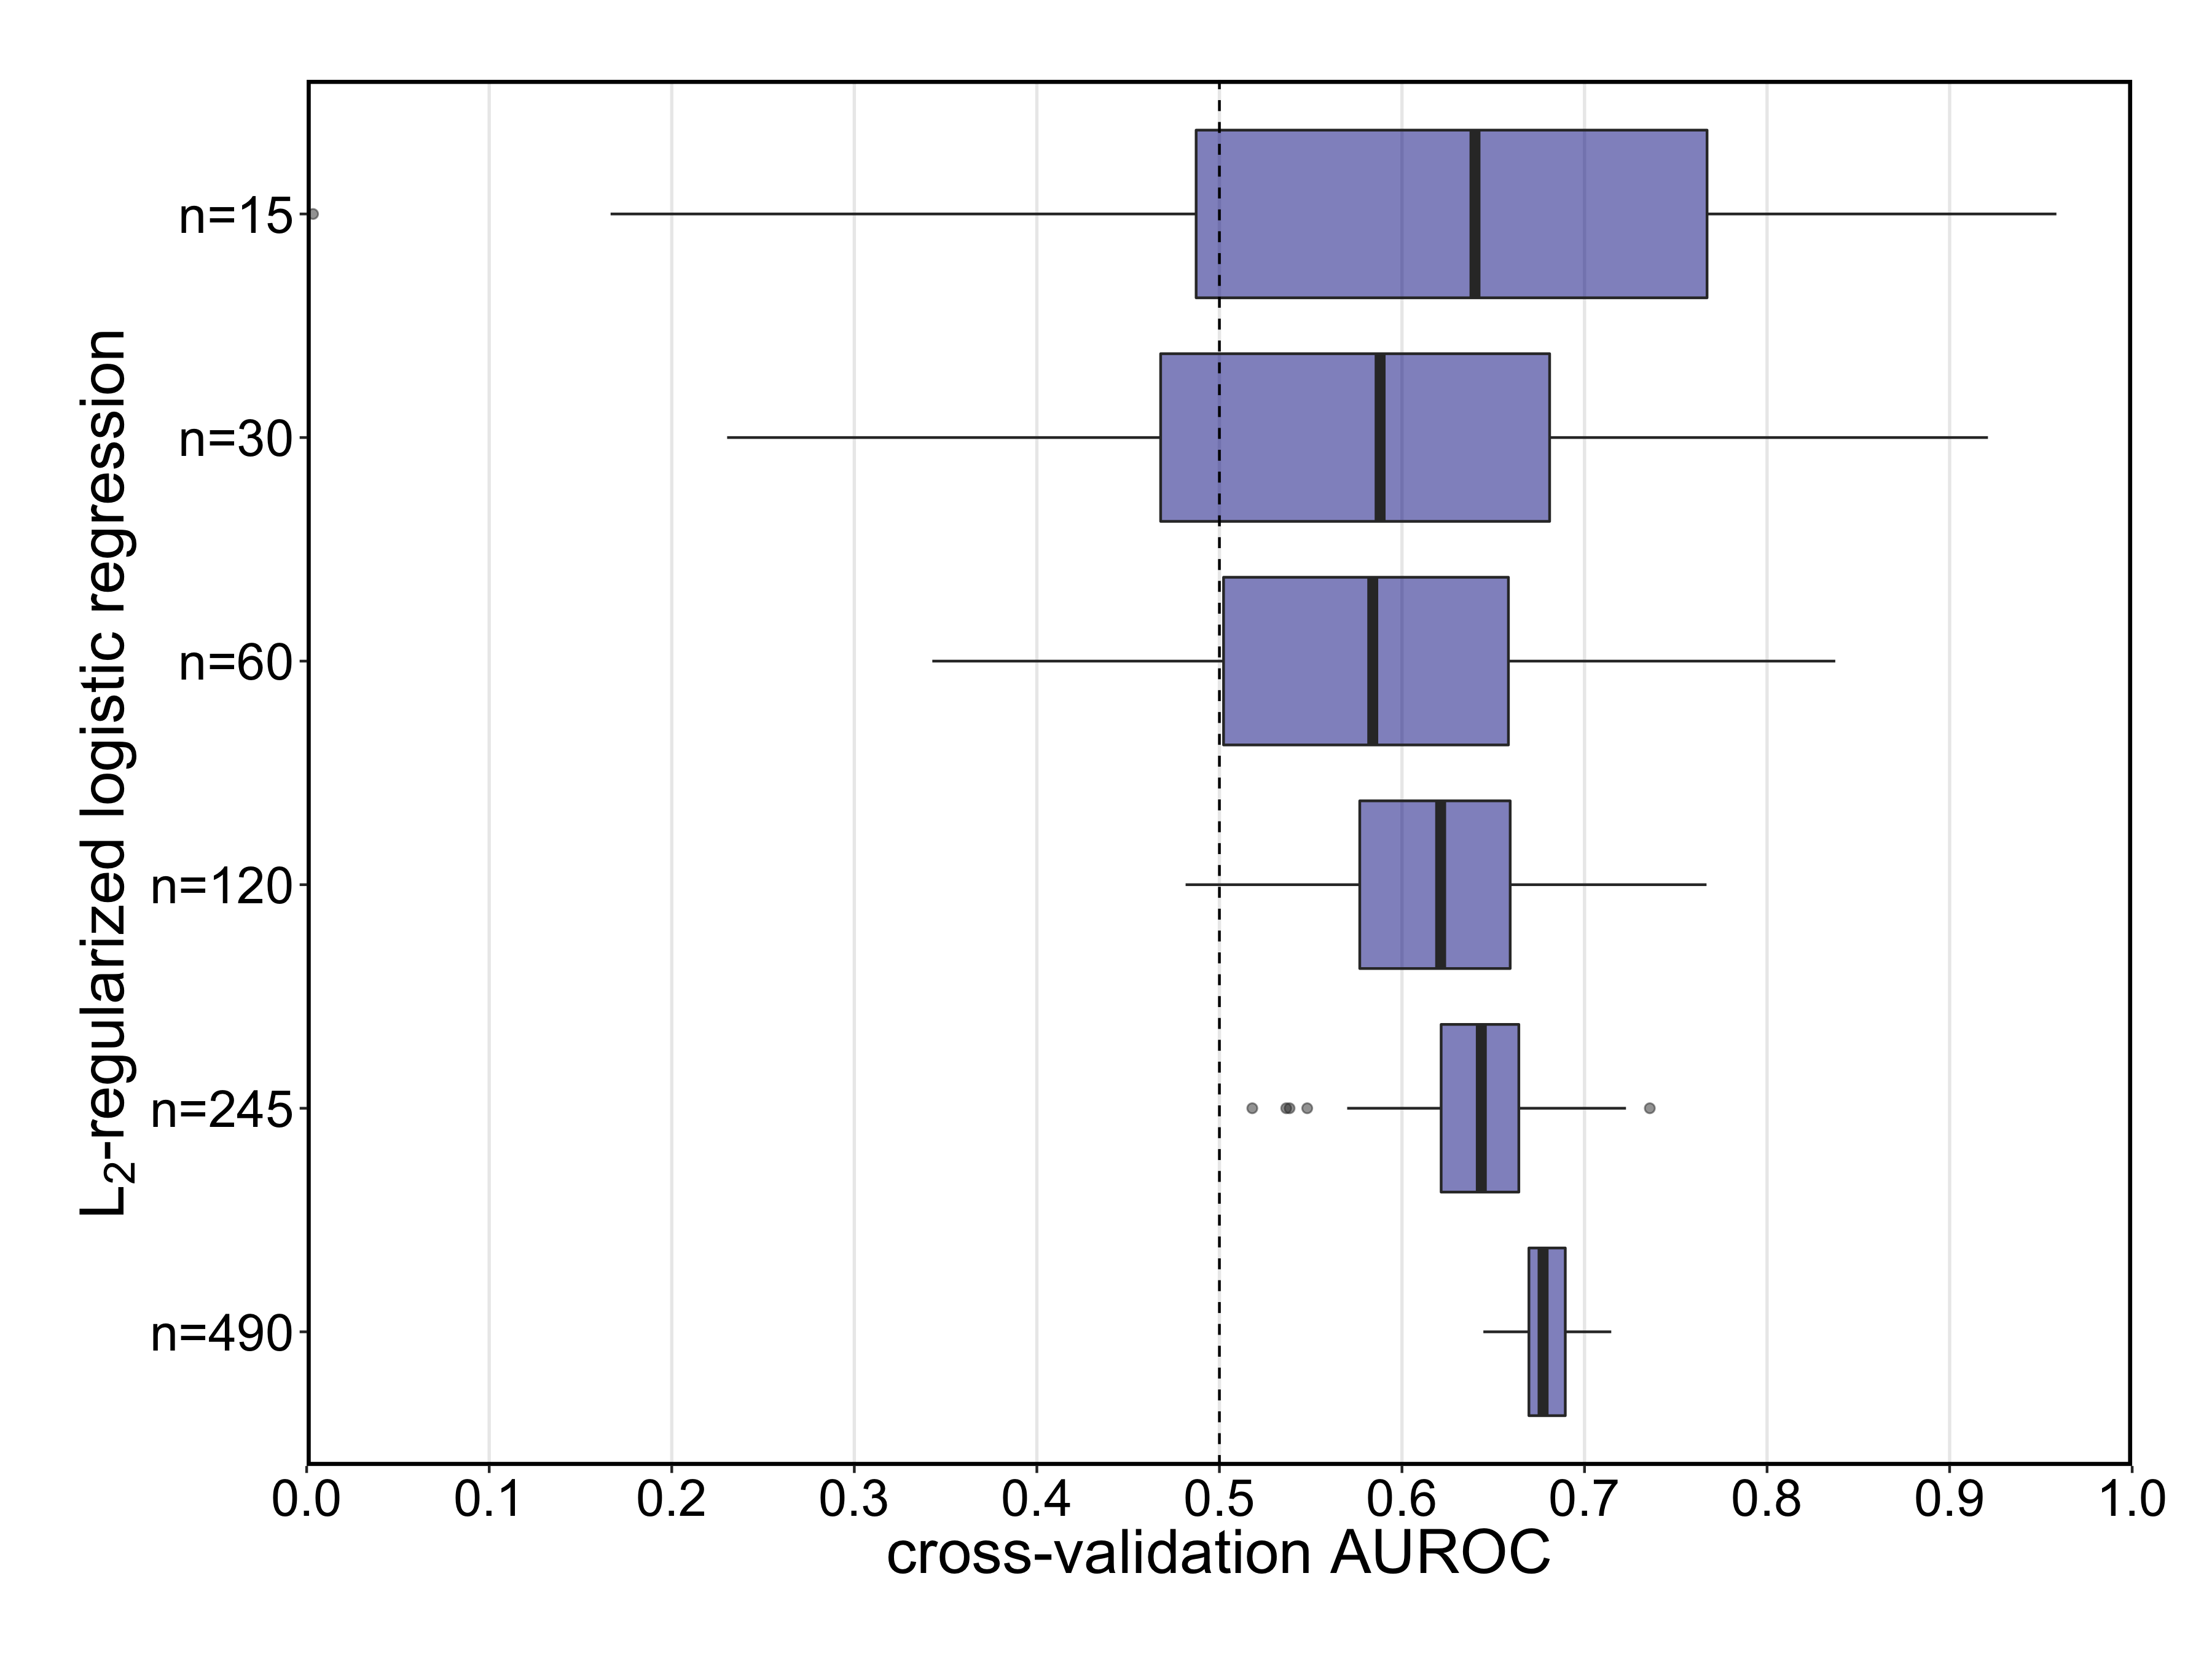
\includegraphics[height=17.5cm, width=13cm]{Figure_S5.png}

\textbf{Figure S5. Interpretation of the linear ML models with
permutation importance.} (A) L1-regularized SVM with linear kernel, (B)
L2-regularized SVM with linear kernel, and (C) L2-regularized logistic
regression were interpreted using permutation importance using held-out
test set.

\newpage

\captionsetup{labelformat=empty}
\captionof{table}{\textbf{Table 1.} Characteristics of the machine learning models in our comparative study.}
\small

\begin{tabular}{|l|l|l|}
\hline

\rowcolor{lightgray}
\textbf{Model} & \textbf{Description} & \textbf{Linearity} \\ \hline

\makecell[l]{Logistic \\regression} & \makecell[l]{A predictive regression analysis when the dependent \\variable is binary.} & Linear \\ \hline

\makecell[l]{SVM with \\linear kernel} & \makecell[l]{A classifier that is defined by an optimal linear \\separating hyperplane that discriminates between labels.} & Linear  \\ \hline

\makecell[l]{SVM with \\radial basis kernel} & \makecell[l]{A classifier that is defined by an optimal non-linear \\separating hyperplane that discriminates between labels.} & Non-linear \\ \hline

\makecell[l]{Decision tree} & \makecell[l]{A classifier that sorts samples down from the
root to the \\leaf node where an attribute is tested to discriminate \\between labels.} & Non-linear \\ \hline

Random forest & \makecell[l]{A classifier that is an ensembe of decision trees \\ that grows randomly with subsampled data.} & Non-linear \\ \hline

\makecell[l]{Gradient Boosted Trees \\ (XGBoost)} & \makecell[l]{A classifier that is an ensembe of decision trees \\ that grows greedily.} & Non-linear \\ \hline

\end{tabular}\newpage

\captionof{table}{\textbf{Table S1.} An aspirational rubric for evaluating the rigor of ML practices.}
\small

\begin{tabular}{|l|l|l|l|}
\hline

\rowcolor{lightgray}
\textbf{Practice} & \textbf{Poor} & \textbf{Good} & \textbf{Better} \\ \hline

\makecell[l]{Source \\ of data} & \makecell[l]{Input data are not appropriate \\ for intended application. \\ (e.g. input data can be \\ used for diagnosis \\ but not prognosis)} & \makecell[l]{Data are generated according \\ to study design and appropriate \\ for intended application} & \makecell[l]{Data are available \\ to predict intended \\ outcomes and will be \\ available in the future } \\ \hline

\makecell[l]{Study \\ cohort} & \makecell[l]{Test data resampled to \\ remove class imbalance} & \makecell[l]{Test data are reflective \\ of the population which \\ the model will eventually \\ be applied to} & \makecell[l]{Model tested on \\ multiple cohorts \\ with different \\ class balances} \\ \hline

\makecell[l]{Model \\ selection} & \makecell[l]{No justification for \\ classification method} & \makecell[l]{Model choice is justified \\ for intended application} & \makecell[l]{Different modeling \\ choices tested} \\ \hline

\makecell[l]{Model \\ development} & \makecell[l]{No hyperparameter tuning} & \makecell[l]{Tested across multiple \\ hyperparameter settings} & \makecell[l]{Cross-validation performed \\ on training set \\ with hyperparameter \\ grid search} \\ \hline

\makecell[l]{Model \\ evaluation} & \makecell[l]{Performance reported on the data \\ used to train the model} & \makecell[l]{Performance reported on \\ held-out test data} & \makecell[l]{Performance reported on \\ multiple held-out test data } \\ \hline

\makecell[l]{Evaluation \\ metrics} & \makecell[l]{Reported a single metric that is \\ not appropriate for intended \\ application  (e.g. when predicting \\ rare outcome, accuracy metric is \\ not reliable)} & \makecell[l]{Reported multiple metrics} & \makecell[l]{Reported multiple metrics \\ with confidence intervals} \\ \hline

\makecell[l]{Model \\ interpretation} & \makecell[l]{No model interpretation} & \makecell[l]{Follow-up analyses to \\ determine what is driving \\ model performance} & \makecell[l]{Hypotheses on important \\ features are generated \\ and tested} \\ \hline

\makecell[l]{Model \\ specification} & \makecell[l]{Only predictive performance \\ reported} & \makecell[l]{Model described \\ (e.g. feature weights)} & \makecell[l]{How to use the model \\ is explained} \\ \hline
\end{tabular}\newpage

\subsection{References}\label{references}

\hypertarget{refs}{}
\hypertarget{ref-segata_metagenomic_2011}{}
1. \textbf{Segata N}, \textbf{Izard J}, \textbf{Waldron L},
\textbf{Gevers D}, \textbf{Miropolsky L}, \textbf{Garrett WS},
\textbf{Huttenhower C}. 2011. Metagenomic biomarker discovery and
explanation. Genome Biol \textbf{12}:R60.
doi:\href{https://doi.org/10.1186/gb-2011-12-6-r60}{10.1186/gb-2011-12-6-r60}.

\hypertarget{ref-zeller_potential_2014}{}
2. \textbf{Zeller G}, \textbf{Tap J}, \textbf{Voigt AY},
\textbf{Sunagawa S}, \textbf{Kultima JR}, \textbf{Costea PI},
\textbf{Amiot A}, \textbf{Böhm J}, \textbf{Brunetti F},
\textbf{Habermann N}, \textbf{Hercog R}, \textbf{Koch M},
\textbf{Luciani A}, \textbf{Mende DR}, \textbf{Schneider MA},
\textbf{Schrotz-King P}, \textbf{Tournigand C}, \textbf{Tran Van Nhieu
J}, \textbf{Yamada T}, \textbf{Zimmermann J}, \textbf{Benes V},
\textbf{Kloor M}, \textbf{Ulrich CM}, \textbf{Knebel Doeberitz M von},
\textbf{Sobhani I}, \textbf{Bork P}. 2014. Potential of fecal microbiota
for early-stage detection of colorectal cancer. Mol Syst Biol
\textbf{10}.
doi:\href{https://doi.org/10.15252/msb.20145645}{10.15252/msb.20145645}.

\hypertarget{ref-zackular_human_2014}{}
3. \textbf{Zackular JP}, \textbf{Rogers MAM}, \textbf{Ruffin MT},
\textbf{Schloss PD}. 2014. The human gut microbiome as a screening tool
for colorectal cancer. Cancer Prev Res \textbf{7}:1112--1121.
doi:\href{https://doi.org/10.1158/1940-6207.CAPR-14-0129}{10.1158/1940-6207.CAPR-14-0129}.

\hypertarget{ref-baxter_dna_2016}{}
4. \textbf{Baxter NT}, \textbf{Koumpouras CC}, \textbf{Rogers MAM},
\textbf{Ruffin MT}, \textbf{Schloss PD}. 2016. DNA from fecal
immunochemical test can replace stool for detection of colonic lesions
using a microbiota-based model. Microbiome \textbf{4}.
doi:\href{https://doi.org/10.1186/s40168-016-0205-y}{10.1186/s40168-016-0205-y}.

\hypertarget{ref-baxter_microbiota-based_2016}{}
5. \textbf{Baxter NT}, \textbf{Ruffin MT}, \textbf{Rogers MAM},
\textbf{Schloss PD}. 2016. Microbiota-based model improves the
sensitivity of fecal immunochemical test for detecting colonic lesions.
Genome Medicine \textbf{8}:37.
doi:\href{https://doi.org/10.1186/s13073-016-0290-3}{10.1186/s13073-016-0290-3}.

\hypertarget{ref-hale_shifts_2017}{}
6. \textbf{Hale VL}, \textbf{Chen J}, \textbf{Johnson S},
\textbf{Harrington SC}, \textbf{Yab TC}, \textbf{Smyrk TC},
\textbf{Nelson H}, \textbf{Boardman LA}, \textbf{Druliner BR},
\textbf{Levin TR}, \textbf{Rex DK}, \textbf{Ahnen DJ}, \textbf{Lance P},
\textbf{Ahlquist DA}, \textbf{Chia N}. 2017. Shifts in the fecal
microbiota associated with adenomatous polyps. Cancer Epidemiol
Biomarkers Prev \textbf{26}:85--94.
doi:\href{https://doi.org/10.1158/1055-9965.EPI-16-0337}{10.1158/1055-9965.EPI-16-0337}.

\hypertarget{ref-pasolli_machine_2016}{}
7. \textbf{Pasolli E}, \textbf{Truong DT}, \textbf{Malik F},
\textbf{Waldron L}, \textbf{Segata N}. 2016. Machine learning
meta-analysis of large metagenomic datasets: Tools and biological
insights. PLoS Comput Biol \textbf{12}.
doi:\href{https://doi.org/10.1371/journal.pcbi.1004977}{10.1371/journal.pcbi.1004977}.

\hypertarget{ref-sze_looking_2016}{}
8. \textbf{Sze MA}, \textbf{Schloss PD}. 2016. Looking for a signal in
the noise: Revisiting obesity and the microbiome. mBio \textbf{7}.
doi:\href{https://doi.org/10.1128/mBio.01018-16}{10.1128/mBio.01018-16}.

\hypertarget{ref-walters_meta-analyses_2014}{}
9. \textbf{Walters WA}, \textbf{Xu Z}, \textbf{Knight R}. 2014.
Meta-analyses of human gut microbes associated with obesity and IBD.
FEBS Lett \textbf{588}:4223--4233.
doi:\href{https://doi.org/10.1016/j.febslet.2014.09.039}{10.1016/j.febslet.2014.09.039}.

\hypertarget{ref-vazquez-baeza_guiding_2018}{}
10. \textbf{Vázquez-Baeza Y}, \textbf{Gonzalez A}, \textbf{Xu ZZ},
\textbf{Washburne A}, \textbf{Herfarth HH}, \textbf{Sartor RB},
\textbf{Knight R}. 2018. Guiding longitudinal sampling in IBD cohorts.
Gut \textbf{67}:1743--1745.
doi:\href{https://doi.org/10.1136/gutjnl-2017-315352}{10.1136/gutjnl-2017-315352}.

\hypertarget{ref-qin_alterations_2014}{}
11. \textbf{Qin N}, \textbf{Yang F}, \textbf{Li A}, \textbf{Prifti E},
\textbf{Chen Y}, \textbf{Shao L}, \textbf{Guo J}, \textbf{Le Chatelier
E}, \textbf{Yao J}, \textbf{Wu L}, \textbf{Zhou J}, \textbf{Ni S},
\textbf{Liu L}, \textbf{Pons N}, \textbf{Batto JM}, \textbf{Kennedy SP},
\textbf{Leonard P}, \textbf{Yuan C}, \textbf{Ding W}, \textbf{Chen Y},
\textbf{Hu X}, \textbf{Zheng B}, \textbf{Qian G}, \textbf{Xu W},
\textbf{Ehrlich SD}, \textbf{Zheng S}, \textbf{Li L}. 2014. Alterations
of the human gut microbiome in liver cirrhosis. Nature
\textbf{513}:59--64.
doi:\href{https://doi.org/10.1038/nature13568}{10.1038/nature13568}.

\hypertarget{ref-geman_deep_2018}{}
12. \textbf{Geman O}, \textbf{Chiuchisan I}, \textbf{Covasa M},
\textbf{Doloc C}, \textbf{Milici M-R}, \textbf{Milici L-D}. 2018. Deep
learning tools for human microbiome big data, pp. 265--275. \emph{In}
Balas, VE, Jain, LC, Balas, MM (eds.), Soft computing applications.
Springer International Publishing.

\hypertarget{ref-thaiss_persistent_2016}{}
13. \textbf{Thaiss CA}, \textbf{Itav S}, \textbf{Rothschild D},
\textbf{Meijer MT}, \textbf{Levy M}, \textbf{Moresi C},
\textbf{Dohnalová L}, \textbf{Braverman S}, \textbf{Rozin S},
\textbf{Malitsky S}, \textbf{Dori-Bachash M}, \textbf{Kuperman Y},
\textbf{Biton I}, \textbf{Gertler A}, \textbf{Harmelin A},
\textbf{Shapiro H}, \textbf{Halpern Z}, \textbf{Aharoni A},
\textbf{Segal E}, \textbf{Elinav E}. 2016. Persistent microbiome
alterations modulate the rate of post-dieting weight regain. Nature
\textbf{540}:544--551.
doi:\href{https://doi.org/10.1038/nature20796}{10.1038/nature20796}.

\hypertarget{ref-dadkhah_gut_2019}{}
14. \textbf{Dadkhah E}, \textbf{Sikaroodi M}, \textbf{Korman L},
\textbf{Hardi R}, \textbf{Baybick J}, \textbf{Hanzel D}, \textbf{Kuehn
G}, \textbf{Kuehn T}, \textbf{Gillevet PM}. 2019. Gut microbiome
identifies risk for colorectal polyps. BMJ Open Gastroenterology
\textbf{6}:e000297.
doi:\href{https://doi.org/10.1136/bmjgast-2019-000297}{10.1136/bmjgast-2019-000297}.

\hypertarget{ref-flemer_oral_2018}{}
15. \textbf{Flemer B}, \textbf{Warren RD}, \textbf{Barrett MP},
\textbf{Cisek K}, \textbf{Das A}, \textbf{Jeffery IB}, \textbf{Hurley
E}, \textbf{O`Riordain M}, \textbf{Shanahan F}, \textbf{O`Toole PW}.
2018. The oral microbiota in colorectal cancer is distinctive and
predictive. Gut \textbf{67}:1454--1463.
doi:\href{https://doi.org/10.1136/gutjnl-2017-314814}{10.1136/gutjnl-2017-314814}.

\hypertarget{ref-montassier_pretreatment_2016}{}
16. \textbf{Montassier E}, \textbf{Al-Ghalith GA}, \textbf{Ward T},
\textbf{Corvec S}, \textbf{Gastinne T}, \textbf{Potel G}, \textbf{Moreau
P}, \textbf{Cochetiere MF de la}, \textbf{Batard E}, \textbf{Knights D}.
2016. Pretreatment gut microbiome predicts chemotherapy-related
bloodstream infection. Genome Medicine \textbf{8}:49.
doi:\href{https://doi.org/10.1186/s13073-016-0301-4}{10.1186/s13073-016-0301-4}.

\hypertarget{ref-ai_systematic_2017}{}
17. \textbf{Ai L}, \textbf{Tian H}, \textbf{Chen Z}, \textbf{Chen H},
\textbf{Xu J}, \textbf{Fang J-Y}. 2017. Systematic evaluation of
supervised classifiers for fecal microbiota-based prediction of
colorectal cancer. Oncotarget \textbf{8}:9546--9556.
doi:\href{https://doi.org/10.18632/oncotarget.14488}{10.18632/oncotarget.14488}.

\hypertarget{ref-dai_multi-cohort_2018}{}
18. \textbf{Dai Z}, \textbf{Coker OO}, \textbf{Nakatsu G}, \textbf{Wu
WKK}, \textbf{Zhao L}, \textbf{Chen Z}, \textbf{Chan FKL},
\textbf{Kristiansen K}, \textbf{Sung JJY}, \textbf{Wong SH}, \textbf{Yu
J}. 2018. Multi-cohort analysis of colorectal cancer metagenome
identified altered bacteria across populations and universal bacterial
markers. Microbiome \textbf{6}:70.
doi:\href{https://doi.org/10.1186/s40168-018-0451-2}{10.1186/s40168-018-0451-2}.

\hypertarget{ref-mossotto_classification_2017}{}
19. \textbf{Mossotto E}, \textbf{Ashton JJ}, \textbf{Coelho T},
\textbf{Beattie RM}, \textbf{MacArthur BD}, \textbf{Ennis S}. 2017.
Classification of paediatric inflammatory bowel disease using machine
learning. Scientific Reports \textbf{7}.
doi:\href{https://doi.org/10.1038/s41598-017-02606-2}{10.1038/s41598-017-02606-2}.

\hypertarget{ref-wong_quantitation_2017}{}
20. \textbf{Wong SH}, \textbf{Kwong TNY}, \textbf{Chow T-C}, \textbf{Luk
AKC}, \textbf{Dai RZW}, \textbf{Nakatsu G}, \textbf{Lam TYT},
\textbf{Zhang L}, \textbf{Wu JCY}, \textbf{Chan FKL}, \textbf{Ng SSM},
\textbf{Wong MCS}, \textbf{Ng SC}, \textbf{Wu WKK}, \textbf{Yu J},
\textbf{Sung JJY}. 2017. Quantitation of faecal fusobacterium improves
faecal immunochemical test in detecting advanced colorectal neoplasia.
Gut \textbf{66}:1441--1448.
doi:\href{https://doi.org/10.1136/gutjnl-2016-312766}{10.1136/gutjnl-2016-312766}.

\hypertarget{ref-statnikov_comprehensive_2013}{}
21. \textbf{Statnikov A}, \textbf{Henaff M}, \textbf{Narendra V},
\textbf{Konganti K}, \textbf{Li Z}, \textbf{Yang L}, \textbf{Pei Z},
\textbf{Blaser MJ}, \textbf{Aliferis CF}, \textbf{Alekseyenko AV}. 2013.
A comprehensive evaluation of multicategory classification methods for
microbiomic data. Microbiome \textbf{1}:11.
doi:\href{https://doi.org/10.1186/2049-2618-1-11}{10.1186/2049-2618-1-11}.

\hypertarget{ref-knights_supervised_2011}{}
22. \textbf{Knights D}, \textbf{Costello EK}, \textbf{Knight R}. 2011.
Supervised classification of human microbiota. FEMS Microbiology Reviews
\textbf{35}:343--359.
doi:\href{https://doi.org/10.1111/j.1574-6976.2010.00251.x}{10.1111/j.1574-6976.2010.00251.x}.

\hypertarget{ref-wirbel_meta-analysis_2019}{}
23. \textbf{Wirbel J}, \textbf{Pyl PT}, \textbf{Kartal E}, \textbf{Zych
K}, \textbf{Kashani A}, \textbf{Milanese A}, \textbf{Fleck JS},
\textbf{Voigt AY}, \textbf{Palleja A}, \textbf{Ponnudurai R},
\textbf{Sunagawa S}, \textbf{Coelho LP}, \textbf{Schrotz-King P},
\textbf{Vogtmann E}, \textbf{Habermann N}, \textbf{Niméus E},
\textbf{Thomas AM}, \textbf{Manghi P}, \textbf{Gandini S},
\textbf{Serrano D}, \textbf{Mizutani S}, \textbf{Shiroma H},
\textbf{Shiba S}, \textbf{Shibata T}, \textbf{Yachida S}, \textbf{Yamada
T}, \textbf{Waldron L}, \textbf{Naccarati A}, \textbf{Segata N},
\textbf{Sinha R}, \textbf{Ulrich CM}, \textbf{Brenner H},
\textbf{Arumugam M}, \textbf{Bork P}, \textbf{Zeller G}. 2019.
Meta-analysis of fecal metagenomes reveals global microbial signatures
that are specific for colorectal cancer. Nature Medicine
\textbf{25}:679.
doi:\href{https://doi.org/10.1038/s41591-019-0406-6}{10.1038/s41591-019-0406-6}.

\hypertarget{ref-vangay_microbiome_2019}{}
24. \textbf{Vangay P}, \textbf{Hillmann BM}, \textbf{Knights D}. 2019.
Microbiome learning repo (ML repo): A public repository of microbiome
regression and classification tasks. Gigascience \textbf{8}.
doi:\href{https://doi.org/10.1093/gigascience/giz042}{10.1093/gigascience/giz042}.

\hypertarget{ref-galkin_human_2018}{}
25. \textbf{Galkin F}, \textbf{Aliper A}, \textbf{Putin E},
\textbf{Kuznetsov I}, \textbf{Gladyshev VN}, \textbf{Zhavoronkov A}.
2018. Human microbiome aging clocks based on deep learning and tandem of
permutation feature importance and accumulated local effects. bioRxiv.
doi:\href{https://doi.org/10.1101/507780}{10.1101/507780}.

\hypertarget{ref-reiman_using_2017}{}
26. \textbf{Reiman D}, \textbf{Metwally A}, \textbf{Dai Y}. 2017. Using
convolutional neural networks to explore the microbiome, pp. 4269--4272.
\emph{In} 2017 39th annual international conference of the IEEE
engineering in medicine and biology society (EMBC).

\hypertarget{ref-fioravanti_phylogenetic_2017}{}
27. \textbf{Fioravanti D}, \textbf{Giarratano Y}, \textbf{Maggio V},
\textbf{Agostinelli C}, \textbf{Chierici M}, \textbf{Jurman G},
\textbf{Furlanello C}. 2017. Phylogenetic convolutional neural networks
in metagenomics. arXiv:170902268 {[}cs, q-bio{]}.

\hypertarget{ref-thomas_metagenomic_2019}{}
28. \textbf{Thomas AM}, \textbf{Manghi P}, \textbf{Asnicar F},
\textbf{Pasolli E}, \textbf{Armanini F}, \textbf{Zolfo M},
\textbf{Beghini F}, \textbf{Manara S}, \textbf{Karcher N}, \textbf{Pozzi
C}, \textbf{Gandini S}, \textbf{Serrano D}, \textbf{Tarallo S},
\textbf{Francavilla A}, \textbf{Gallo G}, \textbf{Trompetto M},
\textbf{Ferrero G}, \textbf{Mizutani S}, \textbf{Shiroma H},
\textbf{Shiba S}, \textbf{Shibata T}, \textbf{Yachida S}, \textbf{Yamada
T}, \textbf{Wirbel J}, \textbf{Schrotz-King P}, \textbf{Ulrich CM},
\textbf{Brenner H}, \textbf{Arumugam M}, \textbf{Bork P}, \textbf{Zeller
G}, \textbf{Cordero F}, \textbf{Dias-Neto E}, \textbf{Setubal JC},
\textbf{Tett A}, \textbf{Pardini B}, \textbf{Rescigno M},
\textbf{Waldron L}, \textbf{Naccarati A}, \textbf{Segata N}. 2019.
Metagenomic analysis of colorectal cancer datasets identifies
cross-cohort microbial diagnostic signatures and a link with choline
degradation. Nature Medicine \textbf{25}:667.
doi:\href{https://doi.org/10.1038/s41591-019-0405-7}{10.1038/s41591-019-0405-7}.

\hypertarget{ref-rudin_please_2018}{}
29. \textbf{Rudin C}. 2018. Please stop explaining black box models for
high stakes decisions. arXiv:181110154 {[}cs, stat{]}.

\hypertarget{ref-rudin_optimized_2018}{}
30. \textbf{Rudin C}, \textbf{Ustun B}. 2018. Optimized scoring systems:
Toward trust in machine learning for healthcare and criminal justice.
Interfaces \textbf{48}:449--466.
doi:\href{https://doi.org/10.1287/inte.2018.0957}{10.1287/inte.2018.0957}.

\hypertarget{ref-knights_human-associated_2011}{}
31. \textbf{Knights D}, \textbf{Parfrey LW}, \textbf{Zaneveld J},
\textbf{Lozupone C}, \textbf{Knight R}. 2011. Human-associated microbial
signatures: Examining their predictive value. Cell Host Microbe
\textbf{10}:292--296.
doi:\href{https://doi.org/10.1016/j.chom.2011.09.003}{10.1016/j.chom.2011.09.003}.

\hypertarget{ref-Ng:2004:FSL:1015330.1015435}{}
32. \textbf{Ng AY}. 2004. Feature selection, l1 vs. l2 regularization,
and rotational invariance, pp. 78. \emph{In} Proceedings of the
twenty-first international conference on machine learning. ACM, New
York, NY, USA.

\hypertarget{ref-miller_explanation_2017}{}
33. \textbf{Miller T}. 2017. Explanation in artificial intelligence:
Insights from the social sciences. arXiv:170607269 {[}cs{]}.

\hypertarget{ref-ribeiro_why_2016}{}
34. \textbf{Ribeiro MT}, \textbf{Singh S}, \textbf{Guestrin C}. 2016.
``Why should i trust you?'': Explaining the predictions of any
classifier. arXiv:160204938 {[}cs, stat{]}.

\hypertarget{ref-nori_interpretml:_2019}{}
35. \textbf{Nori H}, \textbf{Jenkins S}, \textbf{Koch P},
\textbf{Caruana R}. 2019. InterpretML: A unified framework for machine
learning interpretability. arXiv:190909223 {[}cs, stat{]}.

\hypertarget{ref-10.1093ux2fbioinformaticsux2fbtq134}{}
36. \textbf{Altmann A}, \textbf{Toloşi L}, \textbf{Sander O},
\textbf{Lengauer T}. 2010. Permutation importance: a corrected feature
importance measure. Bioinformatics \textbf{26}:1340--1347.
doi:\href{https://doi.org/10.1093/bioinformatics/btq134}{10.1093/bioinformatics/btq134}.

\hypertarget{ref-dormann_collinearity:_2013}{}
37. \textbf{Dormann CF}, \textbf{Elith J}, \textbf{Bacher S},
\textbf{Buchmann C}, \textbf{Carl G}, \textbf{Carré G}, \textbf{Marquéz
JRG}, \textbf{Gruber B}, \textbf{Lafourcade B}, \textbf{Leitão PJ},
\textbf{Münkemüller T}, \textbf{McClean C}, \textbf{Osborne PE},
\textbf{Reineking B}, \textbf{Schröder B}, \textbf{Skidmore AK},
\textbf{Zurell D}, \textbf{Lautenbach S}. 2013. Collinearity: A review
of methods to deal with it and a simulation study evaluating their
performance. Ecography \textbf{36}:27--46.
doi:\href{https://doi.org/10.1111/j.1600-0587.2012.07348.x}{10.1111/j.1600-0587.2012.07348.x}.

\hypertarget{ref-sze_fecal_2019}{}
38. \textbf{Sze MA}, \textbf{Topçuoğlu BD}, \textbf{Lesniak NA},
\textbf{Ruffin MT}, \textbf{Schloss PD}. 2019. Fecal short-chain fatty
acids are not predictive of colonic tumor status and cannot be predicted
based on bacterial community structure. mBio \textbf{10}:e01454--19.
doi:\href{https://doi.org/10.1128/mBio.01454-19}{10.1128/mBio.01454-19}.

\hypertarget{ref-kocheturov_massive_2019}{}
39. \textbf{Kocheturov A}, \textbf{Pardalos PM}, \textbf{Karakitsiou A}.
2019. Massive datasets and machine learning for computational
biomedicine: Trends and challenges. Ann Oper Res \textbf{276}:5--34.
doi:\href{https://doi.org/10.1007/s10479-018-2891-2}{10.1007/s10479-018-2891-2}.

\hypertarget{ref-kim_improved_2018}{}
40. \textbf{Kim M}, \textbf{Oh I}, \textbf{Ahn J}. 2018. An improved
method for prediction of cancer prognosis by network learning. Genes
\textbf{9}:478.
doi:\href{https://doi.org/10.3390/genes9100478}{10.3390/genes9100478}.

\hypertarget{ref-wiens_no_2019}{}
41. \textbf{Wiens J}, \textbf{Saria S}, \textbf{Sendak M},
\textbf{Ghassemi M}, \textbf{Liu VX}, \textbf{Doshi-Velez F},
\textbf{Jung K}, \textbf{Heller K}, \textbf{Kale D}, \textbf{Saeed M},
\textbf{Ossorio PN}, \textbf{Thadaney-Israni S}, \textbf{Goldenberg A}.
2019. Do no harm: A roadmap for responsible machine learning for health
care. Nat Med \textbf{25}:1337--1340.
doi:\href{https://doi.org/10.1038/s41591-019-0548-6}{10.1038/s41591-019-0548-6}.

\hypertarget{ref-westcott_opticlust_2017}{}
42. \textbf{Westcott SL}, \textbf{Schloss PD}. 2017. OptiClust, an
Improved Method for Assigning Amplicon-Based Sequence Data to
Operational Taxonomic Units. mSphere \textbf{2}.
doi:\href{https://doi.org/10.1128/mSphereDirect.00073-17}{10.1128/mSphereDirect.00073-17}.

\hypertarget{ref-redwood_stool_2016}{}
43. \textbf{Redwood DG}, \textbf{Asay ED}, \textbf{Blake ID},
\textbf{Sacco PE}, \textbf{Christensen CM}, \textbf{Sacco FD},
\textbf{Tiesinga JJ}, \textbf{Devens ME}, \textbf{Alberts SR},
\textbf{Mahoney DW}, \textbf{Yab TC}, \textbf{Foote PH}, \textbf{Smyrk
TC}, \textbf{Provost EM}, \textbf{Ahlquist DA}. 2016. Stool DNA testing
for screening detection of colorectal neoplasia in alaska native people.
Mayo Clin Proc \textbf{91}:61--70.
doi:\href{https://doi.org/10.1016/j.mayocp.2015.10.008}{10.1016/j.mayocp.2015.10.008}.

\hypertarget{ref-sze_leveraging_2018}{}
44. \textbf{Sze MA}, \textbf{Schloss PD}. 2018. Leveraging existing 16S
rRNA gene surveys to identify reproducible biomarkers in individuals
with colorectal tumors. mBio \textbf{9}:e00630--18.
doi:\href{https://doi.org/10.1128/mBio.00630-18}{10.1128/mBio.00630-18}.

\hypertarget{ref-schloss_introducing_2009}{}
45. \textbf{Schloss PD}, \textbf{Westcott SL}, \textbf{Ryabin T},
\textbf{Hall JR}, \textbf{Hartmann M}, \textbf{Hollister EB},
\textbf{Lesniewski RA}, \textbf{Oakley BB}, \textbf{Parks DH},
\textbf{Robinson CJ}, \textbf{Sahl JW}, \textbf{Stres B},
\textbf{Thallinger GG}, \textbf{Van Horn DJ}, \textbf{Weber CF}. 2009.
Introducing mothur: Open-Source, Platform-Independent,
Community-Supported Software for Describing and Comparing Microbial
Communities. ApplEnvironMicrobiol \textbf{75}:7537--7541.

\hypertarget{ref-rognes_vsearch_2016}{}
46. \textbf{Rognes T}, \textbf{Flouri T}, \textbf{Nichols B},
\textbf{Quince C}, \textbf{Mahé F}. 2016. VSEARCH: A versatile open
source tool for metagenomics. PeerJ \textbf{4}:e2584.
doi:\href{https://doi.org/10.7717/peerj.2584}{10.7717/peerj.2584}.

\hypertarget{ref-li_hyperband:_2016}{}
47. \textbf{Li L}, \textbf{Jamieson K}, \textbf{DeSalvo G},
\textbf{Rostamizadeh A}, \textbf{Talwalkar A}. 2016. Hyperband: A novel
bandit-based approach to hyperparameter optimization. arXiv:160306560
{[}cs, stat{]}.


\end{document}
